

%%%%%%%%%%%%%%%%%%%%%%%%%%%%%%%%%%%%%%%%
% datoteka diploma.tex

\documentclass[a4paper, 12pt]{book}
%\documentclass[a4paper, 12pt, draft]{book}  Nalogo preverite tudi z opcijo draft, ki vam bo pokazala, katere vrstice so predolge!



\usepackage[utf8x]{inputenc}   % omogoča uporabo slovenskih črk kodiranih v formatu UTF-8
\usepackage[slovene,english]{babel}    % naloži, med drugim, slovenske delilne vzorce
\usepackage[pdftex]{graphicx}  % omogoča vlaganje slik različnih formatov
\usepackage{fancyhdr}          % poskrbi, na primer, za glave strani
\usepackage{amssymb}           % dodatni simboli
\usepackage{amsmath}           % eqref, npr.
%\usepackage{hyperxmp}
\usepackage[hyphens]{url}  % dodal Solina
\usepackage{comment}       % dodal Solina

\usepackage[pdftex, colorlinks=true,
						citecolor=black, filecolor=black, 
						linkcolor=black, urlcolor=black,
						pagebackref=false, 
						pdfproducer={LaTeX}, pdfcreator={LaTeX}, hidelinks]{hyperref}

\usepackage{color}       % dodal Solina
\usepackage{soul}       % dodal Solina

%%%%%%%%%%%%%%%%%%%%%%%%%%%%%%%%%%%%%%%%
%	CUSTOME
%%%%%%%%%%%%%%%%%%%%%%%%%%%%%%%%%%%%%%%%
\usepackage{array}
\usepackage{tabularx}
\usepackage{listings}
\usepackage{xcolor}


\renewcommand{\lstlistingname}{Koda}
\renewcommand{\lstlistlistingname}{Seznam kod}

\newcolumntype{b}{X}
\newcolumntype{s}{>{\hsize=.9\hsize}X}
\newcolumntype{z}{>{\hsize=.2\hsize}X}

\definecolor{codegreen}{rgb}{0,0.6,0}
\definecolor{codegray}{rgb}{0.5,0.5,0.5}
\definecolor{codepurple}{rgb}{0.20,0,0.82}
\definecolor{backcolour}{rgb}{0.97,0.97,0.97}

\lstdefinestyle{mystyle}{
    backgroundcolor=\color{backcolour},   
    commentstyle=\color{codegreen},
    keywordstyle=\color{magenta},
    numberstyle=\tiny\color{codegray},
    stringstyle=\color{codepurple},
    basicstyle=\ttfamily\footnotesize,
    breakatwhitespace=false,         
    breaklines=true,                 
    captionpos=b,                    
    keepspaces=true,                 
    numbers=left,                    
    numbersep=5pt,                  
    showspaces=false,                
    showstringspaces=false,
    showtabs=false,                  
    tabsize=2
}


% %%%%%%%%%%%%%%%%%%%%%%%%%%%%%%%%%%%%%%%%
% %	DIPLOMA INFO
% %%%%%%%%%%%%%%%%%%%%%%%%%%%%%%%%%%%%%%%%
\newcommand{\ttitle}{Spletni pregled in urejanje raziskovalnih in drugih publikacij}
\newcommand{\ttitleEn}{Online review and editing of research and other publications}
\newcommand{\tsubject}{\ttitle}
\newcommand{\tsubjectEn}{\ttitleEn}
\newcommand{\tauthor}{Žiga Marolt}
\newcommand{\tkeywords}{spletna aplikacija, publikacije, Vue.js, docker, OpenApi}
\newcommand{\tkeywordsEn}{web application, publicitations, Vue.js, docker, OpenApi}


%%%%%%%%%%%%%%%%%%%%%%%%%%%%%%%%%%%%%%%%
%	HYPERREF SETUP
%%%%%%%%%%%%%%%%%%%%%%%%%%%%%%%%%%%%%%%%
\hypersetup{pdftitle={\ttitle}}
\hypersetup{pdfsubject=\ttitleEn}
\hypersetup{pdfauthor={\tauthor, zm1218@student.uni-lj.si}}
\hypersetup{pdfkeywords=\tkeywordsEn}

 


%%%%%%%%%%%%%%%%%%%%%%%%%%%%%%%%%%%%%%%%
% postavitev strani
%%%%%%%%%%%%%%%%%%%%%%%%%%%%%%%%%%%%%%%%  

\addtolength{\marginparwidth}{-20pt} % robovi za tisk
\addtolength{\oddsidemargin}{40pt}
\addtolength{\evensidemargin}{-40pt}

\renewcommand{\baselinestretch}{1.3} % ustrezen razmik med vrsticami
\setlength{\headheight}{15pt}        % potreben prostor na vrhu
\renewcommand{\chaptermark}[1]%
{\markboth{\MakeUppercase{\thechapter.\ #1}}{}} \renewcommand{\sectionmark}[1]%
{\markright{\MakeUppercase{\thesection.\ #1}}} \renewcommand{\headrulewidth}{0.5pt} \renewcommand{\footrulewidth}{0pt}
\fancyhf{}
\fancyhead[LE,RO]{\sl \thepage} 
\fancyhead[LO]{\sl \rightmark} \fancyhead[RE]{\sl \leftmark}
% \fancyhead[RE]{\sc \tauthor}              % dodal Solina
% \fancyhead[LO]{\sc Diplomska naloga}     % dodal Solina


\newcommand{\BibTeX}{{\sc Bib}\TeX}

%%%%%%%%%%%%%%%%%%%%%%%%%%%%%%%%%%%%%%%%
% naslovi
%%%%%%%%%%%%%%%%%%%%%%%%%%%%%%%%%%%%%%%%  


\newcommand{\autfont}{\Large}
\newcommand{\titfont}{\LARGE\bf}
\newcommand{\clearemptydoublepage}{\newpage{\pagestyle{empty}\cleardoublepage}}
\setcounter{tocdepth}{2}	      % globina kazala

%%%%%%%%%%%%%%%%%%%%%%%%%%%%%%%%%%%%%%%%
% konstrukti
%%%%%%%%%%%%%%%%%%%%%%%%%%%%%%%%%%%%%%%%  
\newtheorem{izrek}{Izrek}[chapter]
\newtheorem{trditev}{Trditev}[izrek]
\newenvironment{dokaz}{\emph{Dokaz.}\ }{\hspace{\fill}{$\Box$}}

%%%%%%%%%%%%%%%%%%%%%%%%%%%%%%%%%%%%%%%%%%%%%%%%%%%%%%%%%%%%%%%%%%%%%%%%%%%%%%%
%% PDF-A
%%%%%%%%%%%%%%%%%%%%%%%%%%%%%%%%%%%%%%%%%%%%%%%%%%%%%%%%%%%%%%%%%%%%%%%%%%%%%%%


%%%%%%%%%%%%%%%%%%%%%%%%%%%%%%%%%%%%%%%% 
% define medatata
%%%%%%%%%%%%%%%%%%%%%%%%%%%%%%%%%%%%%%%% 
\def\Title{\ttitle}
\def\Author{\tauthor, matjaz.kralj@fri.uni-lj.si}
\def\Subject{\ttitleEn}
\def\Keywords{\tkeywordsEn}

%%%%%%%%%%%%%%%%%%%%%%%%%%%%%%%%%%%%%%%% 
% \convertDate converts D:20080419103507+02'00' to 2008-04-19T10:35:07+02:00
%%%%%%%%%%%%%%%%%%%%%%%%%%%%%%%%%%%%%%%% 
\def\convertDate{%
    \getYear
}

{\catcode`\D=12
 \gdef\getYear D:#1#2#3#4{\edef\xYear{#1#2#3#4}\getMonth}
}
\def\getMonth#1#2{\edef\xMonth{#1#2}\getDay}
\def\getDay#1#2{\edef\xDay{#1#2}\getHour}
\def\getHour#1#2{\edef\xHour{#1#2}\getMin}
\def\getMin#1#2{\edef\xMin{#1#2}\getSec}
\def\getSec#1#2{\edef\xSec{#1#2}\getTZh}
\def\getTZh +#1#2{\edef\xTZh{#1#2}\getTZm}
\def\getTZm '#1#2'{%
    \edef\xTZm{#1#2}%
    \edef\convDate{\xYear-\xMonth-\xDay T\xHour:\xMin:\xSec+\xTZh:\xTZm}%
}

\expandafter\convertDate\pdfcreationdate 

%%%%%%%%%%%%%%%%%%%%%%%%%%%%%%%%%%%%%%%%
% get pdftex version string
%%%%%%%%%%%%%%%%%%%%%%%%%%%%%%%%%%%%%%%% 
\newcount\countA
\countA=\pdftexversion
\advance \countA by -100
\def\pdftexVersionStr{pdfTeX-1.\the\countA.\pdftexrevision}


%%%%%%%%%%%%%%%%%%%%%%%%%%%%%%%%%%%%%%%%
% XMP data
%%%%%%%%%%%%%%%%%%%%%%%%%%%%%%%%%%%%%%%%  
\usepackage{xmpincl}
\includexmp{pdfa-1b}

%%%%%%%%%%%%%%%%%%%%%%%%%%%%%%%%%%%%%%%%
% pdfInfo
%%%%%%%%%%%%%%%%%%%%%%%%%%%%%%%%%%%%%%%%  
\pdfinfo{%
    /Title    (\ttitle)
    /Author   (\tauthor, zm1218@student.uni-lj.si)
    /Subject  (\ttitleEn)
    /Keywords (\tkeywordsEn)
    /ModDate  (\pdfcreationdate)
    /Trapped  /False
}


%%%%%%%%%%%%%%%%%%%%%%%%%%%%%%%%%%%%%%%%%%%%%%%%%%%%%%%%%%%%%%%%%%%%%%%%%%%%%%%
%%%%%%%%%%%%%%%%%%%%%%%%%%%%%%%%%%%%%%%%%%%%%%%%%%%%%%%%%%%%%%%%%%%%%%%%%%%%%%%

\begin{document}
\selectlanguage{slovene}
\frontmatter
\setcounter{page}{1} %
\renewcommand{\thepage}{}       % preprecimo težave s številkami strani v kazalu
\newcommand{\sn}[1]{"`#1"'}                    % dodal Solina (slovenski narekovaji)

%%%%%%%%%%%%%%%%%%%%%%%%%%%%%%%%%%%%%%%%
%naslovnica
 \thispagestyle{empty}%
  \begin{center}
    {\large\sc Univerza v Ljubljani\\%
      Fakulteta za računalništvo in informatiko}%
    \vskip 10em%
    {\autfont \tauthor\par}%
    {\titfont \ttitle \par}%
    {\vskip 3em \textsc{DIPLOMSKO DELO\\[5mm]       
    VISOKOŠOLSKI STROKOVNI ŠTUDIJSKI PROGRAM\\ PRVE STOPNJE\\ RAČUNALNIŠTVO IN INFORMATIKA}\par}%
    \vfill\null%
    {\large \textsc{Mentor}: doc.\ dr.  Mira Trebar\par}%
    {\vskip 2em \large Ljubljana, 2022 \par}%
\end{center}
% prazna stran
%\clearemptydoublepage      % dodal Solina (izjava o licencah itd. se izpiše na hrbtni strani naslovnice)

%%%%%%%%%%%%%%%%%%%%%%%%%%%%%%%%%%%%%%%%
%copyright stran
\thispagestyle{empty}
\vspace*{8cm}

\noindent
{\sc Copyright}. 
Rezultati diplomske naloge so intelektualna lastnina avtorja in Fakultete za računalništvo in informatiko Univerze v Ljubljani.
Za objavo in koriščenje rezultatov diplomske naloge je potrebno pisno privoljenje avtorja, Fakultete za računalništvo in informatiko ter mentorja.

\begin{center}
\mbox{}\vfill
\emph{Besedilo je oblikovano z urejevalnikom besedil \LaTeX.}
\end{center}
% prazna stran
\clearemptydoublepage

%%%%%%%%%%%%%%%%%%%%%%%%%%%%%%%%%%%%%%%%
% stran 3 med uvodnimi listi
\thispagestyle{empty}
\vspace*{4cm}

\noindent
Fakulteta za računalništvo in informatiko izdaja naslednjo nalogo:
\medskip
\begin{tabbing}
\hspace{32mm}\= \hspace{6cm} \= \kill

Tematika naloge:
\end{tabbing}
Kandidat naj v diplomskem delu implementira spletno rešitev za vnos različ-\\nih publikacij in dodatnih vsebin z namenom urejanja in pregledovanja pomembnih informacij. Predlagana rešitev naj bo zasnovana tako, da imajo prijavljeni uporabniki dostop do podatkov, urednik skrbi za vnos in urejanje, administrator pa ima celovit nadzor nad delovanjem. Uporaba aplikacije naj bo predstavljena za objavljene publikacije in pomembne podatke s področja živil.
\vspace{15mm}


\vspace{2cm}

% prazna stran
\clearemptydoublepage

% zahvala
\thispagestyle{empty}\mbox{}\vfill\null\it%
\noindent
Zahvaljujem se mentorici doc. dr. Miri Trebar za vso pomoč in družini za podporo.
\rm\normalfont

% prazna stran
\clearemptydoublepage

%%%%%%%%%%%%%%%%%%%%%%%%%%%%%%%%%%%%%%%%
% posvetilo, če sama zahvala ne zadošča :-)
% \thispagestyle{empty}\mbox{}{\vskip0.20\textheight}\mbox{}\hfill\begin{minipage}{0.55\textwidth}%
% Svoji dragi Alenčici.
% \normalfont\end{minipage}

% % prazna stran
% \clearemptydoublepage


%%%%%%%%%%%%%%%%%%%%%%%%%%%%%%%%%%%%%%%%
% kazalo
\pagestyle{empty}
\def\thepage{}% preprecimo tezave s stevilkami strani v kazalu
\tableofcontents{}


% prazna stran
\clearemptydoublepage

%%%%%%%%%%%%%%%%%%%%%%%%%%%%%%%%%%%%%%%%
% seznam kratic

\chapter*{Seznam uporabljenih kratic}  % spremenil Solina, da predolge vrstice ne gredo preko desnega roba

\noindent \begin{tabular}{p{0.2\textwidth}|p{.35\textwidth}|p{.35\textwidth}}    % po potrebi razširi prvo kolono tabele na račun drugih dveh!
  {\bf kratica} & {\bf angleško}                             & {\bf slovensko} \\ \hline
  {\bf API} & Application Programming Interface & aplikacijski programski vmesnik \\
  {\bf CSS} & Cascading Style Sheets & predloge za izgled spletnih strani \\
  {\bf ER diagram} & Entity Relationship Diagram & entitetno relacijski diagram \\
  {\bf EB} & Exabyte & Eksabajt \\
  {\bf HTML} & Hyper Text Markup Language & označevalni jezik za izdelavo spletnih strani \\
  {\bf HTTP} & Hyper Text Transfer Protocol & komunikacijski spletni protokol \\
  {\bf IAAA} & Identification, Authentication, Authorization and Accounting & varnostni koncepti: identifikacija, avtentikacija, avtorizacija in odgovornost \\
  {\bf JSON} & JavaScript Object Notation & objektna notacija za JavaScript \\
  {\bf REST} & Representational state transfer & predstavitveni prenos stanja \\
  {\bf SQL} & Structured Query Language & strukturiran poizvedovalni jezik \\
  {\bf URL} & Uniform Resource Locator & enolični krajevnik vira \\
\end{tabular}


% prazna stran
\clearemptydoublepage

%%%%%%%%%%%%%%%%%%%%%%%%%%%%%%%%%%%%%%%%
% povzetek
\addcontentsline{toc}{chapter}{Povzetek}
\chapter*{Povzetek}

\noindent\textbf{Naslov:} \ttitle
\bigskip

\noindent\textbf{Avtor:} \tauthor
\bigskip

%\noindent\textbf{Povzetek:} 
\noindent Dandanes se na spletu pojavlja vedno več raziskovalnih metod iz področja analize in napovedovanja dobe uporabnosti hitro pokvarljivih živil. Vsaka raziskovalna metoda lahko pri raziskovanju uporablja različne parametre. Parametri se razlikujejo glede na format, strukturo ali pa samo vrsto podatkov. 

Namen te diplomske naloge je izdelati spletno aplikacijo s primerno podatkovno shemo za pregled in urejanje publikacij. Preko nje je mogoče dodajati, urejati, brisati in iskati po vnesenih metodah in drugih podatkih. Dostop do posameznih delov aplikacije je dovoljen le določenim uporabnikom z ustreznimi uporabniškimi pravicami. Predstavljen je celoten proces načrtovanja in implementacije aplikacije, ki je zasnovana kot mikrostoritev v programskem jeziku Go. Podane so zahteve, ki jih je potrebno upoštevati pri zasnovi arhitekture spletne aplikacije iz vidika varnosti podatkov, hitrosti razvoja aplikacije in hitrosti same aplikacije. Aplikacija je predstavljena s primerom uporabe testnih podatkov.

\bigskip

\noindent\textbf{Ključne besede:} \tkeywords.
% prazna stran
\clearemptydoublepage

%%%%%%%%%%%%%%%%%%%%%%%%%%%%%%%%%%%%%%%%
% abstract
\selectlanguage{english}
\addcontentsline{toc}{chapter}{Abstract}
\chapter*{Abstract}

\noindent\textbf{Title:} \ttitleEn
\bigskip

\noindent\textbf{Author:} \tauthor
\bigskip

%\noindent\textbf{Abstract:} 
\noindent Nowadays, more and more research methods are appearing in the field of analysis and prediction of perishable foods shelf-life. Each research method may use different parameters in its research. The parameters vary according to format, structure or just the type of data.

The aim of this thesis is to develop a web-based application with a suitable data structure to allow for reviewing and editing the publications. Through the application it is possible to add, edit, delete and search through the entered methods and other data. Access to individual parts of the application is restricted to specific users with the appropriate user rights. Presented here is the complete design process and implementation of the application, which is designed as a microservice in the Go programming language. Given are requirements to be taken into account in the design of the web application architecture in terms of data security, development time and the speed of the application itself. The application is presented with an example using test data.
\bigskip

\noindent\textbf{Keywords:} \tkeywordsEn.
\selectlanguage{slovene}
% prazna stran
\clearemptydoublepage

%%%%%%%%%%%%%%%%%%%%%%%%%%%%%%%%%%%%%%%%
\mainmatter
\setcounter{page}{1}
\pagestyle{fancy}


\chapter{Uvod}

Poleg splošnih informacij je eden od najpomembnejših podatkov, ki so na voljo za posamezna živila, predvsem za hitro pokvarljiva, zapis o roku uporabnosti. Podaja nam informacijo, koliko časa lahko neko živilo hranimo, da varnost in kakovost izdelka ostaneta v sprejemljivem območju. Ob tem morajo biti upoštevani specifični pogoji transporta in shranjevanja. Določitev roka uporabnosti živila temelji na predpostavki, da z živilom ustrezno ravnamo.

Iz dneva v dan nam je na voljo vedno več objavljenih raziskav iz področja ravnanja z živili v preskrbovalni verigi. Raziskave so objavljene v različnih virih, naj si bo to članek na svetovnem spletu, v reviji ali pa v znanstveni knjigi. Raziskovalci, ki prebirajo raziskave pogosto porabijo veliko časa, da pridobijo zanesljive vire in iz njih uspejo pridobiti pomembne in zanesljive informacije.

Da bi poenostavili pridobivanje informacij, smo v diplomski nalogi zasnovali in implementirali aplikacijo za vnos in pregled raziskovalnih publikacij s področja analize in napovedovanja dobe uporabnosti hitro pokvarljivih živil. Aplikacija je zasnovana kot mikrostoritev. Za razvojno okolje je uporabljena Docker arhitektura, kar nam omogoča enostavno postavitev projekta, in pa tudi enostavno objavljanje projekta v izbranem okolju. 

Ker se struktura podatkov razlikuje od raziskave do raziskave in od vira do vira, je pomembno, da podatkovno strukturo pravilno definiramo. Za dobro uporabniško izkušnjo mora biti vnos podatkov o raziskavah enostaven in dosleden, iskanje po le-teh pa mora biti hitro in uporabno. Definirali smo več vrst uporabnikov, ki imajo različne dostope do posameznih delov aplikacije.

V diplomski nalogi bomo predstavili kako smo pristopili k reševanju omenjenega problema, kakšen je bil proces dela in sam razvoj aplikacije. Na koncu bomo spoznali še končno rešitev in samo implementacijo.


% \section{Motivacija}


% Priznajmo si, večina spletnih aplikacij ne rešuje težkih tehničnih izzivov. Pomembno je, da z izdelkom pridemo na trg pred našo konkurenco, zato pa je pomembno, da je izdelek pravilno tehnično strukturiran.
% Morda se to sprva sliši dolgočasno, vendar sam mislim, da je podpirati ta cilj težje, kot se sliši.


\chapter{Razvoj aplikacije}
\label{pregled-podrocja-chapter}

Pred izdelavo diplomskega dela smo najprej na spletu preverili ali obstajajo podobne rešitve na trgu. S tem smo razmislili ali je problem sploh smiseln in vreden razvoja. Med raziskavo smo odkrili nekaj orodij, ki so podobna naši aplikaciji. To so Food Safety Centre \cite{food-safety-centre}, Mendeley \cite{mendeley-manager} in pa Zotero \cite{zotero-manager}. Omenjena orodja nam do neke mere olajšajo delo z organizacijo publikacij, vendar pa nobeno popolnoma ne ustreza našim zahtevam. 


% #####################################################################
\section{Življenjski cikel razvoja }
Razvoj programske opreme je proces, ki je sestavljen iz vrste načrtovanih dejavnosti ali sprememb. Življenjski cikel razvoja je drugačen za vsak projekt, zato je potrebno izbrati primeren model, ki omogoča boljši pregled nad samim procesom razvoja programske opreme, kot tudi testiranja in definiranja le-te.

Za razvoj aplikacije smo uporabili \sn{slapovni model} (ang. waterfall model). Omenjena metodologija je linearni model, pri katerem napredek pretežno teče v eno smer navzdol skozi faze zbiranja potreb, analize, načrtovanja, razvoja, testiranja, uvajanja in vzdrževanja. Izraz je bil prvič uveden v dokumentu, ki ga je leta 1970 objavil dr. Winston W. Royce, in se še naprej uporablja v aplikacijah industrijskega oblikovanja \cite{waterfall-model}.

Omenjeni model je definiran z zaporedjem posameznih faz, katerih število je lahko različno glede na izvedbo metodologije, giblje pa se med pet in sedem različnimi fazami (Slika \ref{waterfall-phases}). Izhod ene faze se uporablja kot vhod naslednje faze, torej mora biti vsaka faza zaključena, preden se lahko začne naslednja.

\begin{description}
    \item \textbf{Opis posameznih faz:}
    \begin{enumerate}
        \item \textbf{Zbiranje zahtev} – vse možne zahteve so zajete v dokumentih z opisom izdelka.
        \item \textbf{Analiziranje} - pregled specifikacij in analiziranje le-teh. Z analiziranjem se definira poslovno logiko in pa tudi finančni plan projekta.
        \item \textbf{Zasnova sistema} - glede na predhodno analizo se načrtuje arhitekturo programske opreme.
        \item \textbf{Izvedba} - razvoj programske opreme v manjših enotah s funkcionalnim testiranjem.
        \item \textbf{Integracija in testiranje} - integracija vsake enote, razvite v prejšnji fazi in po integraciji, katerim sledi testiranje celotnega sistema za morebitne napake.
        \item \textbf{Uvedba sistema} – po opravljenih vseh funkcionalnih in nefunkcionalnih testiranjih izdelek deluje v proizvodnem okolju.
        \item \textbf{Vzdrževanje} - odpravljanje težav in izdaja nove različice s popravki se izvaja po potrebi.
    \end{enumerate}
\end{description}

Zaradi medsebojne odvisnosti posameznih faz je model pri implementaciji zelo pregleden in jasen. Vendar ima nekaj pomanjkljivosti in je učinkovit le pri manjših projektih, kjer so zahteve zelo jasno definirane in kjer je predviden obseg dela manjši.
Model ne dovoljuje spreminjanja specifikacij, oziroma je spreminjanje zahtev med samo implementacijo oteženo. Ko je izdelek v fazi testiranja, se je težko vrniti in spremeniti nekaj, kar je ostalo v fazi analize.
To pomeni, da delujoč izdelek dobimo šele na koncu cikla omenjenega modela. 

\begin{figure}[h]
\begin{center}
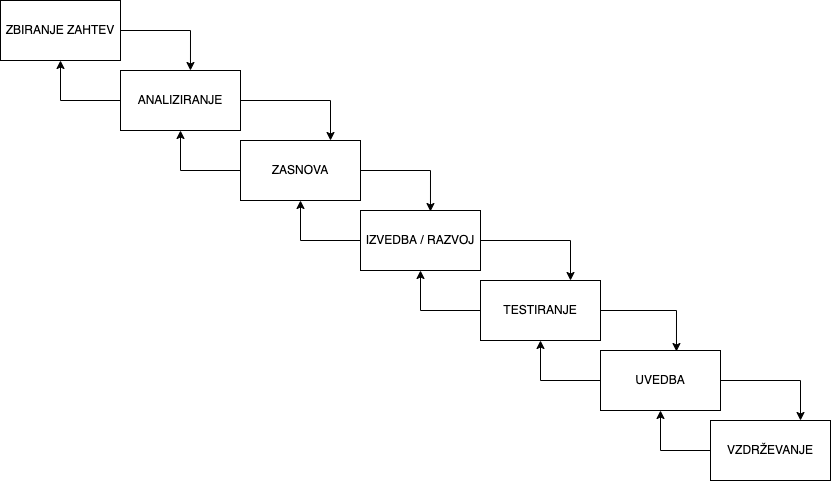
\includegraphics[width=0.9\textwidth]{slike/waterfall.png}
\end{center}
\caption{ Vizualizacija sedmih faz slapovnega modela }
\label{waterfall-phases}
\end{figure}

% #####################################################################
\section{Pregled zahtev}
Cilj izdelave spletne aplikacije je agregirati podatke iz različnih virov, kot so knjiga, spletni vir ali pa revija. Vnašanje omenjenih podatkov iz nedefiniranih virov je težko in zamudno opravilo. Aplikacija mora biti razvita z namenom, da je uporabniku, ki publikacije vnaša v sistem, delo olajšano. 

Aplikacija naj omogoča vnos novih in urejanje obstoječih publikacij. Vsak vnos mora biti pred objavo potrjen s strani administratorja. vnesene publikacije naj bodo primerno prikazane končnemu uporabniku, z možnostjo iskanja po posameznih zapisih. 

% Urednikom in administratorjem mora biti omogočeno dodajanje novih parametrov za posamezno publikacijo, z možnostjo hitrega iskanja po vrednostih parametrov med samim dodajanjem publikacije. 

Aplikacija mora biti pregledna in enostavna za uporabo. Podpirati mora registracijo novih uporabnikov v aplikacijo in omejiti dostop do določene vsebine glede na vlogo uporabnika. Dostop do posameznih strani naj bo omogočen le prijavljenim uporabnikom z uporabniškim imenom in geslom ter primernim dostopom (Slika \ref{user-rights}). Definirani uporabniki so: 
\begin{itemize}
    \item \textbf{Uporabnik} - omogočen je pregled objavljenih publikacij in pripadajočih vsebin.
	\item \textbf{Urednik} - lahko ureja publikacije, vsebine ter parametre za posamezno publikacijo.
	\item \textbf{Administrator} - ima polni nadzor aplikacije.
\end{itemize}

\begin{figure}[h]
\begin{center}
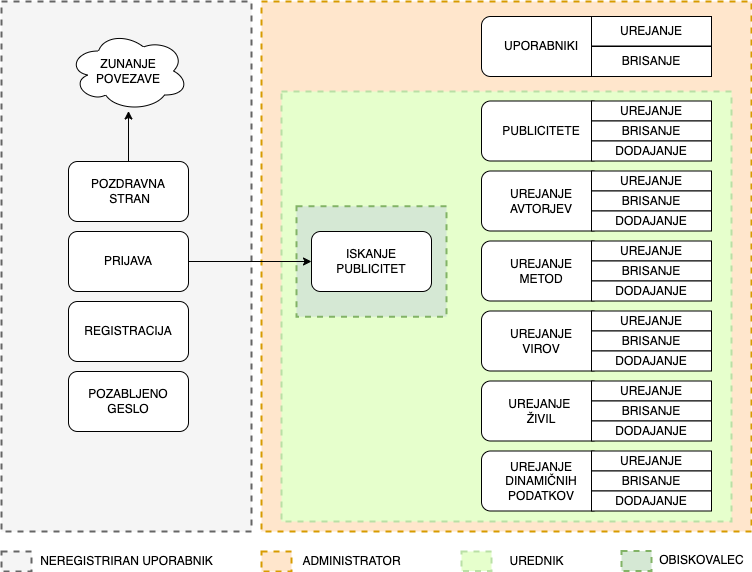
\includegraphics[width=0.75\textwidth]{slike/user_hierarchy.png}
\end{center}
\caption{ Pregled dostopa do posameznih strani in akcij glede na vlogo uporabnika }
\label{user-rights}
\end{figure}

Zaledni sistem naj bo zasnovan tako, da ga bo mogoče nadgraditi in kasneje uporabiti v mobilni aplikaciji. Uporabniški vmesnik aplikacije naj bo v angleščini, komunikacija med čelnim in zalednim sistemom pa naj bo ustrezno dokumentirana.

% \section{Funkcionalnosti}


% prazna stran
% ===================
% RAZVOJ APLIKACIJE
% ===================
\section{Načrtovanje aplikacije}
\label{nacrtovanje}
%% @ziga "razdelali strukturo strani" - nejasen pomen besede "strani" - manjka kak pridevnik?
Na podlagi zahtev smo začeli z načrtovanjem aplikacije. Najprej smo popisali vse funkcionalnosti, katere mora aplikacija zajemati in razdelali strukturo strani. Glede na popisane funkcionalnosti smo se odločili kako bo projekt postavljen in definirali arhitekturo aplikacije. 

Med načrtovanjem smo se odločili tudi kateri programski jezik bomo uporabili. Definirali smo kako bo potekala komunikacija med posameznimi internimi storitvami in komunikacijo med zalednim in čelnim delom. 

V nadaljevanju bomo spoznali posamezne tehnologije in metode, uporabljene pri razvoju aplikacije in čemu je katera tehnologija namenjena. 

% +++++++++++++++++++++++++++++++++++++++++++++
\subsection{Funkcionalnosti in njihove povezave}
Aplikacija je sestavljena iz sklopov strani, do katerih lahko dostopamo iz različnih delov aplikacije. Za lažjo predstavitev so na sliki \ref{sitemap} prikazane povezave med posameznimi stranmi, med katerimi se uporabnik lahko premika. Opisi zahtev za posamezne strani so naslednji:


\begin{figure}[h]
\begin{center}
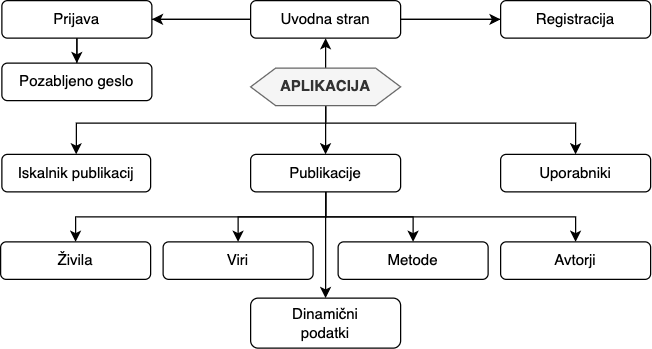
\includegraphics[width=0.9\textwidth]{slike/page-map.png}
\end{center}
\caption{ Zemljevid aplikacije (ang. sitemap). }
\label{sitemap}
\end{figure}


\begin{description}
        \item \textbf{Registracija}: ustvarjanje novega uporabnika
		\item \textbf{Prijava}: obrazec za overjanje uporabnika
		\item \textbf{Pozabljeno geslo}: nastavitev novega gesla uporabniku
		\item \textbf{Uporabniki}: seznam vseh uporabnikov
		\begin{itemize}
		    \item urejanje: obrazec za urejanje uporabnika
		    \item brisanje: deaktiviranje uporabnika
		\end{itemize}
		\item \textbf{Publikacije}: seznam vnesenih publikacij
		\begin{itemize}
		    \item urejanje: obrazec za urejanje obstoječe publikacije
		    \item brisanje: odstranitev publikacije
		    \item dodajanje: obrazec za kreiranje nove publikacije
		    \item iskanje: iskanje po naslovu 
		    \item prenos datoteke: prenos pripete datoteke k publikaciji
		\end{itemize}
		\item \textbf{Metode}: seznam vseh vnesenih metod
		\begin{itemize}
		    \item urejanje: obrazec za urejanje obstoječe metode
		    \item brisanje: odstranitev metode
		    \item dodajanje: obrazec za kreiranje nove metode
		\end{itemize}
		
		\item \textbf{Viri}: seznam vseh dodanih virov
		\begin{itemize}
		    \item urejanje: obrazec za urejanje obstoječega vira
		    \item brisanje: odstranitev vira
		    \item dodajanje: obrazec za kreiranje novega vira
		\end{itemize}
		
		\item \textbf{Živila}: seznam vseh dodanih živil
		\begin{itemize}
		    \item urejanje: obrazec za urejanje obstoječega živila
		    \item brisanje: odstranitev živila
		    \item dodajanje: obrazec za kreiranje novega živila
		\end{itemize}
		
		\item \textbf{Avtorji}: seznam vseh dodanih avtorjev
		\begin{itemize}
		    \item urejanje: obrazec za urejanje obstoječega avtorja
		    \item brisanje: odstranitev avtorja
		    \item dodajanje: obrazec za kreiranje novega avtorja
		\end{itemize}
		
		\item \textbf{Dinamični podatki}: seznam vseh definiranih dinamičnih podatkov
		\begin{itemize}
		    \item urejanje: obrazec za urejanje obstoječih podatkov
		    \item brisanje: odstranitev podatka
		    \item dodajanje: obrazec za kreiranje vnosa novih podatkov
		\end{itemize}
		
		\item \textbf{Iskalnik}: stran za iskanje po publikacijah
\end{description}

\subsection{Postavitev spletne strani}
Osnovno postavitev posameznih strani smo najprej skicirali na list papirja. Odločili smo se za postavitev, ki se v spletnih aplikacijah zelo pogosto uporablja in je enostavna in pregledna.

Na vrhu strani se nahaja navigacija, katere namen je premikanje med posameznimi sklopi. Na skrajnem levem delu se nahaja ime aplikacije \sn{Safe Food}. Na skrajnem desnem delu se nahaja gumb za nadzor nad uporabniškim delom. Na sredini navigacije pa se nahajajo povezave do posameznih sklopov aplikacije.

Na strani, kjer uporabnik pregleduje in išče publikacije, smo se odločili, da stran razdelimo na dva dela. Na levem delu strani se nahaja nabor filtrov, na desnem delu pa prikaz publikacij (Slika \ref{wireframe}). 

Vse strani uporabljajo enak koncept. Za enostavno premikanje med stranmi se na dnu nahaja paginacija. V primeru napake pri vnosu podatkov se ta prikaže poleg vnosnega polja. V primeru generalne napake, kot je na primer neuspešno poslan zahtevek na zaledni sistem, pa se ta izpiše na dnu strani v posebnem oknu.

\begin{figure}[h]
\begin{center}
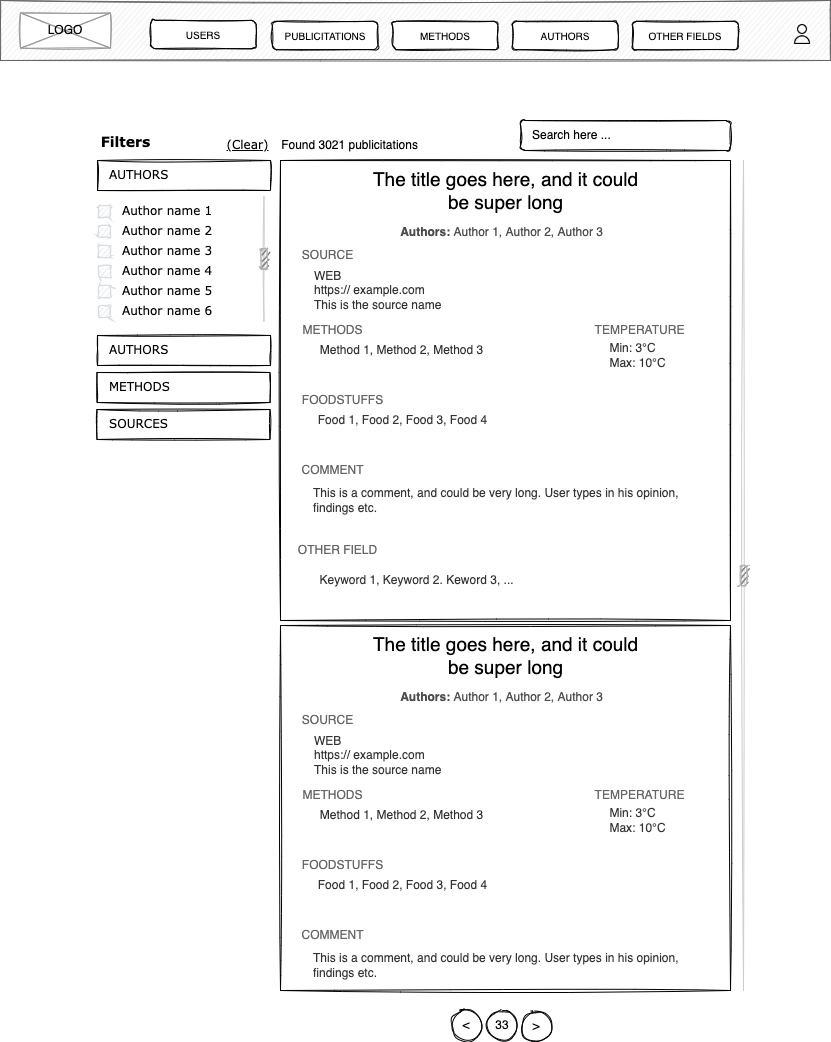
\includegraphics[width=1\textwidth]{slike/wireframe.png}
\end{center}
\caption{ Skica postavitve strani s publikacijami (ang. wireframe). }
\label{wireframe}
\end{figure}

\clearpage

\section{Spletne tehnologije}
\subsection{Nadzor različic}
\label{version-control}
Orodje, ki upravlja in sledi različnim verzijam programske kode ali drugih podatkov, je poznano kot sistem za verzioniranje podatkov. V angleščini poznamo več izrazov, ki se navezujejo na omenjeno orodje, to so Version Control System (VCS), Source Code Manager (SCM) in Revision Control System (RCS). Nadzor različic, znan tudi kot nadzor vira, je praksa sledenja in upravljanja sprememb programske kode. Sistem običajno hrani kodo na dogovorjeni lokaciji na centralnem strežniku (primer GitHub). Razvijalci delajo na svojih lokalnih kopijah izvorne kode, ki jih pridobijo iz centralnega repozitorija. Svoje spremembe pošiljajo na centralni strežnik, pri čemer sistem omogoča tudi reševanje konfliktov, ko dva ali več razvijalcev poskuša poslati na strežnik spremembe istega dela posamične datoteke. Sistem omogoča obnavljanje stanja izvorne kode iz poljubne verzije v preteklosti.

V našem projektu smo se odločili uporabiti sistem za verzioniranje kode Git. Je distribuiran sistem s poudarkom na hitrosti, integriteti podatkov in podpira vzporedne nelinearne tokove dela. Predstavljen je bil leta 2005, za potrebo razvoja Linuxovega jedra iz strani Linux razvijalcev \cite{git-history} in je postal najbolj razširjen sistem na tem področju. Git repozitorij gostujemo na brezplačnem ponudniku omenjene storitve - GitHub (Slika \ref{github-project}). Poleg brezplačnega gostovanja ponuja tudi vrsto drugih rešitev, kot je na primer beleženje dela (ang. "Task Management"), neprekinjeno integracijo (ang. ''Continuous Integration") in vrsto drugih integracij.

\begin{figure}[h]
\begin{center}
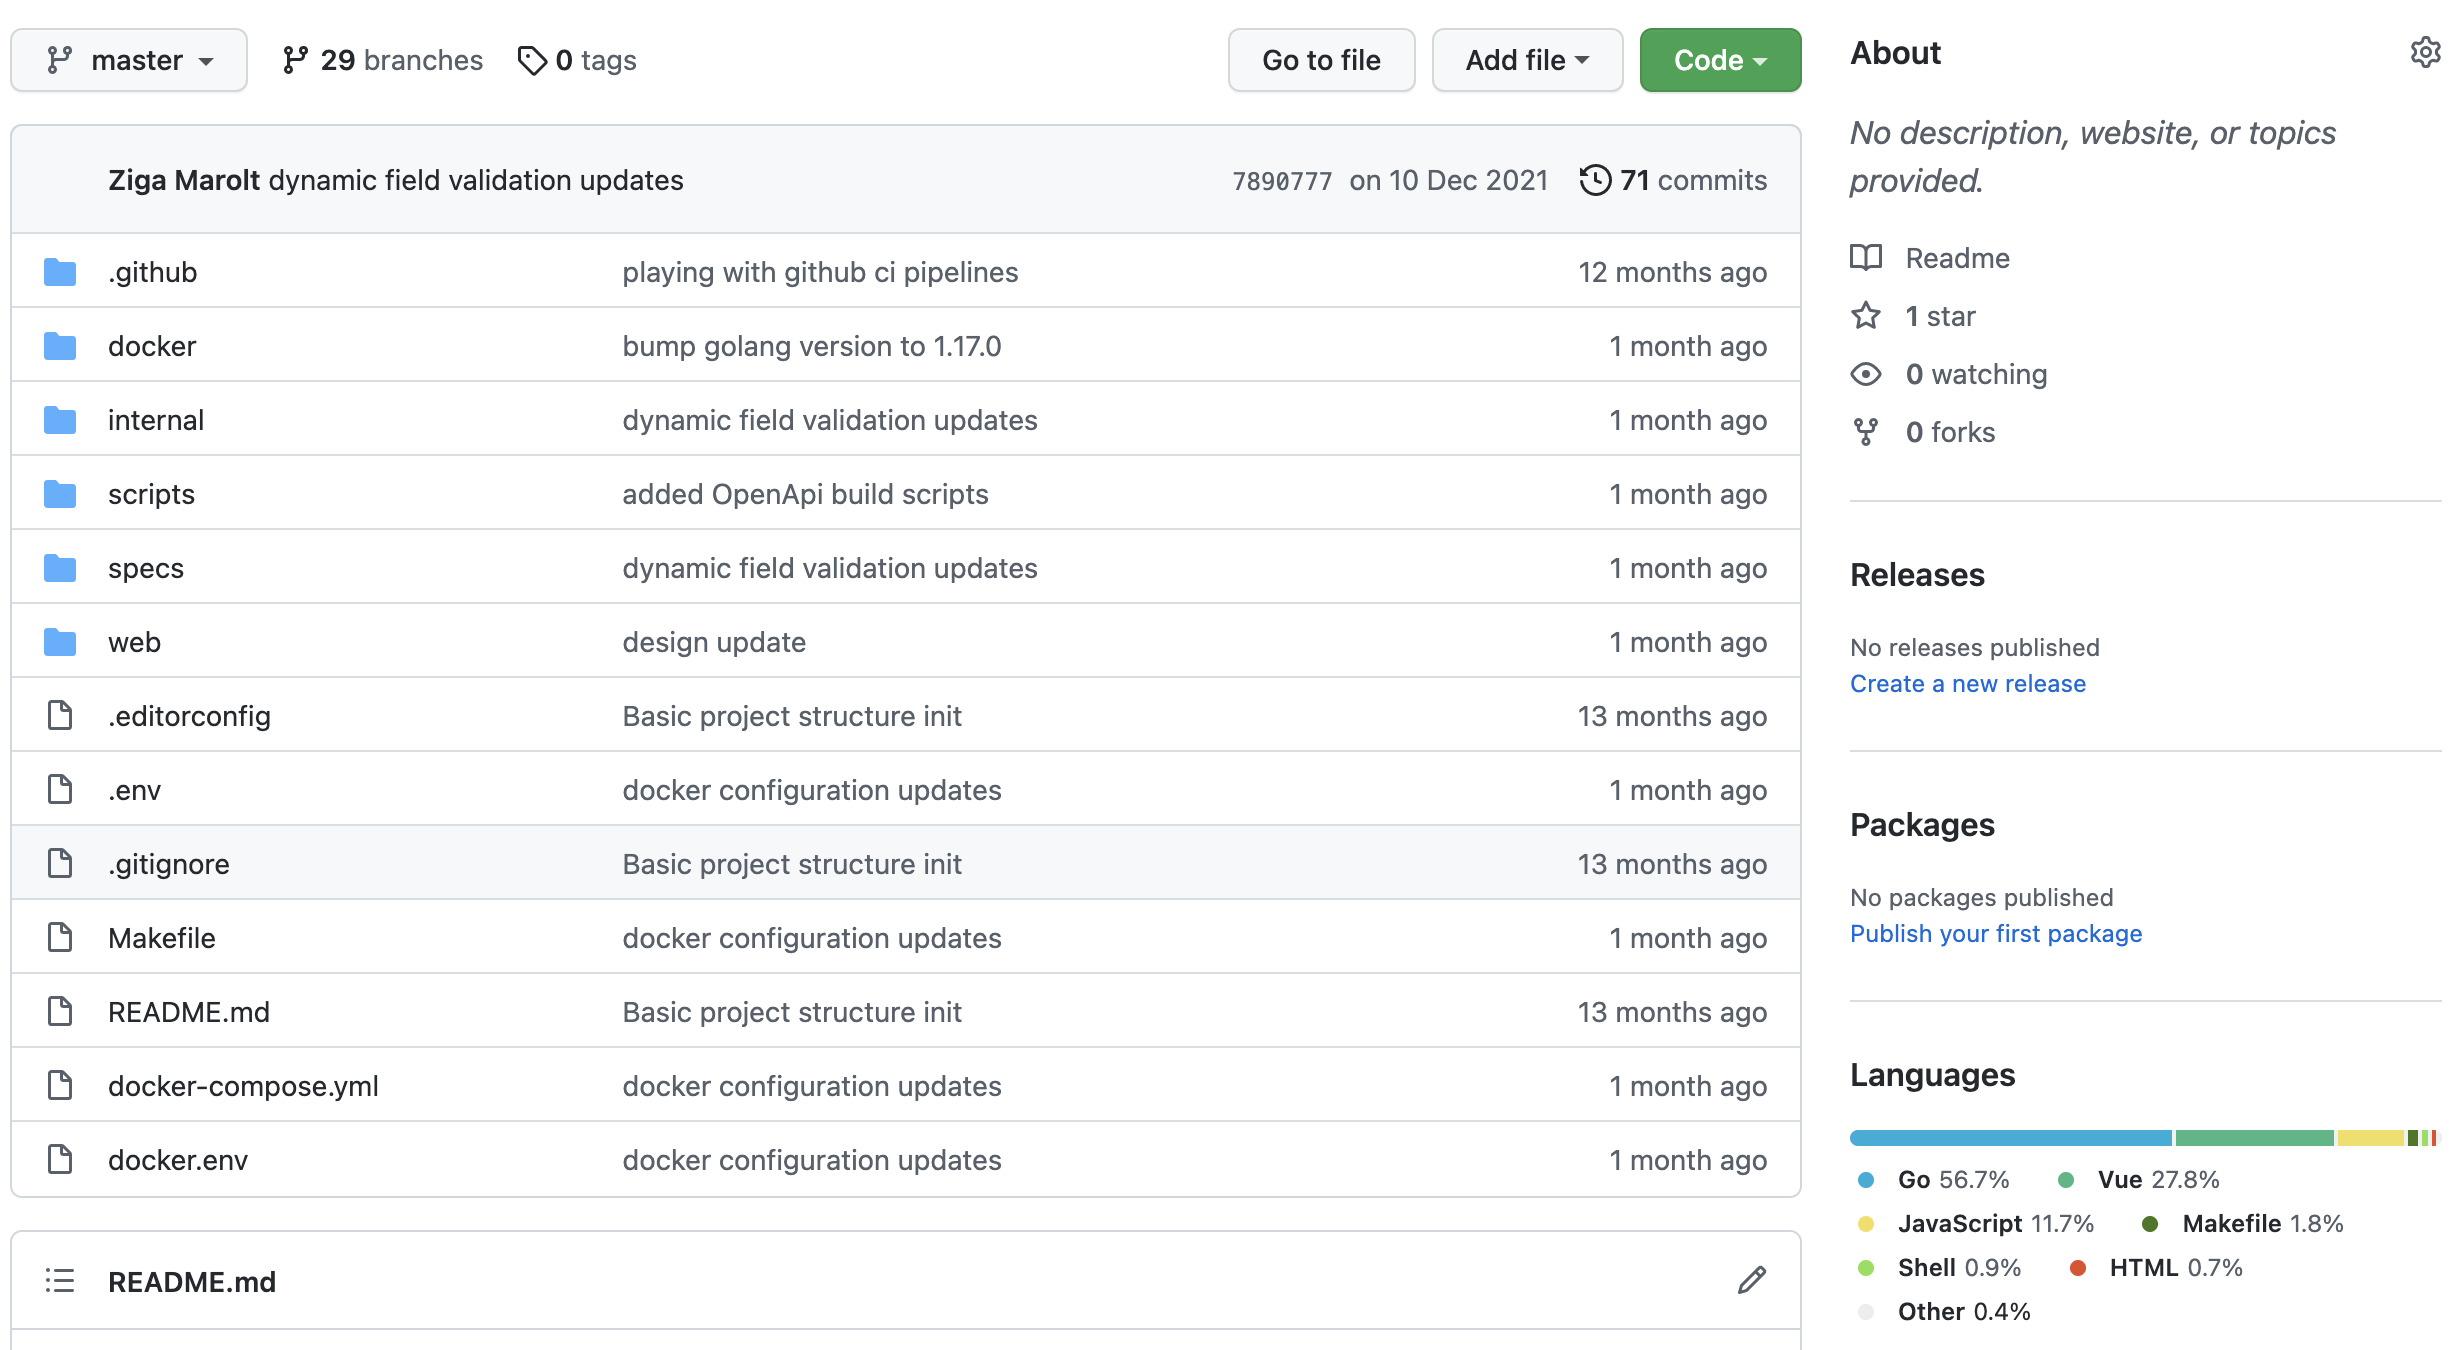
\includegraphics[width=1\textwidth]{slike/github.png}
\end{center}
\caption{ Prikaz GitHub repozitorija }
\label{github-project}
\end{figure}

% #####################################################################
\subsection{Infrastruktura}
Uporaba programske opreme je zapletena. Pred namestitvijo je potrebno razmisliti, kateri operacijski sistem se bo uporabljal, katera so orodja, ki jih programska oprema potrebuje in še vrsto drugih vprašanj. Večina računalnikov že ima nameščene in zagnane aplikacije, ki so odvisne od drugih aplikacij. V primeru, da nekatere aplikacije med seboj niso kompatibilne, lahko pride do težav, ki jih ni enostavno odpraviti. Stvari postanejo bolj zapletene, če si aplikacije med seboj delijo skupne vire. 

Na našem projektu smo se hoteli izogniti nevšečnostim s postavljanjem projekta, zato smo se odločili uporabiti orodje za izoliranje okolja. Virtualizacija je postopek, ki strojni ali programski vir preslika v navidezni vir, tega pa potem odjemalec koristi kot pravi vir. Pomembna prednost uporabe virtualizacije je prenosljivost. Z njo lahko dosežemo enake pogoje za izvajanje programske opreme na različnih strojnih opremah \cite{docker-in-action}.

Orodje Docker zagotavlja tako imenovano abstrakcijo, ki nudi enako okolje vsem razvijalcem, ki razvijajo na istem projektu, ne glede na to, kateri operacijski sistem uporabljajo. Vsebniki (ang. containers) uporabljajo jedra operacijskega sistema in se obnašajo kot navadni programi, ki lahko uporabljajo vse sistemske vire, vendar omejijo dostop aplikacije samo na prostor v vsebnikih (Slika \ref{docker-vs-vm}). \clearpage

\begin{figure}[h]
\begin{center}
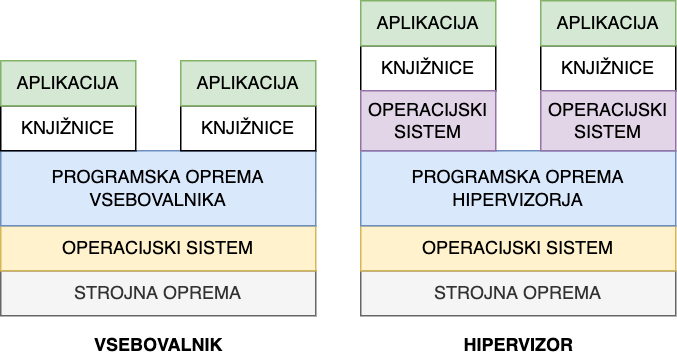
\includegraphics[width=0.75\textwidth]{slike/docker-vs-vm.png}
\end{center}
\caption{ Prikaz razlike med virtualnim strojem in Docker vsebnikom. }
\label{docker-vs-vm}
\end{figure}

% #####################################################################
\subsubsection{Docker}
\label{docker-section}
Docker je trenutno najbolj priljubljena rešitev vsebnika. Ponuja številne funkcije in je podprt s strani ostalih sistemov, kot so na primer orodja za orkestracijo (ang. orchestration). V osnovi gre za izolacijo procesov in virtualizacijo virov, do katerih procesi dostopajo. Omogoča izoliranje aplikacije od infrastrukture, za hitro dostavljanje programske opreme \cite{linuxcontainers}. 
%% @ziga "Omogoča izoliranje aplikacije od infrastrukture, za hitro dostavljanje programske opreme" - nejasno

Docker je odvisen od jedra Linuxa, kar pomeni, da ne deluje v sistemu Windows ali macOS. V tem primeru je potreben zagon v virtualnem stroju, ki vsebuje jedro Linuxa \cite{docker-in-action}.

Konfiguriranje slike vsebnika zahteva ustvarjanje konfiguracijske datoteke. Ta je ponavadi znotraj projekta in se imenuje \sn{Dockerfile}. To je tekstovna datoteka, ki opisuje zahteve posameznega programa, kot so osnovna slika za izvajanje (npr. slika ki omogoča izvajanje Go programov), ukazi za zagon (npr. namestitev), vrata na katerih bo aplikacija poslušala in tako naprej (Slika \ref{docker-flow}).

\begin{figure}[h]
\begin{center}
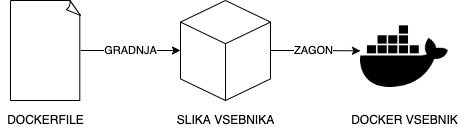
\includegraphics[width=0.75\textwidth]{slike/docker-flow.png}
\end{center}
\caption{ Prikaz gradnje Docker vsebnikov }
\label{docker-flow}
\end{figure}

Vsebnik je skupina procesov v operacijskem sistemu z jedrom Linux, ki upravlja računske vire z nadzornimi skupinami in zagotavlja izolacijo virov z uporabo imenskih prostorov. Ob zagonu vsebnika se uporabi vsebniška slika (angl. container image), v kateri so zapisane informacije o izvajanju programske opreme in preko katere Docker tudi priklopi nov, prazen bralno-pisalni datotečni sloj. Slika se ustvari s postopkom gradnje, ki je zapisan v datoteki $Dockerfile$. 

V kodi \ref{lst:dcb-snipet} je prikazan primer grajenja slike, ki smo jo uporabili pri razvoju zalednega dela naše aplikacije.
\begin{lstlisting}[language=bash, style=mystyle,caption={Grajenje slike Docker vmesnika},label=lst:dcb-snipet]
$ docker build .          
[+] Building 69.1s (9/9)                             FINISHED
 => [internal] load build definition from Dockerfile    0.1s
 => => transferring dockerfile: 180B                    0.0s
 => [internal] load .dockerignore                       0.0s
 => => transferring context: 2B                         0.0s
 => [internal] load metadata for golang:1.17            2.7s
 => [1/2] FROM golang:1.17@sha256:39953c7c7             60.0s
 => => resolve golang:1.17@sha256:39953c7c7             0.0s
 => => sha256:0e29546d54 54.92MB / 54.92MB              27.2s
 => => extracting sha256:0e29546d541                    4.5s
 => => sha256:6432567af305a4304605a3 154B / 154B        34.4s
 => [internal] load build context                       0.0s
 => => transferring context: 121B                       0.0s
 => [2/2] COPY start.sh /                               0.0s 
 => exporting to image                                  0.2s 
 => => exporting layers                                 0.2s 
 => => writing image sha256:96d781a9030                 0.0s 
\end{lstlisting}

% ##################################################################### 
\subsection{Spletni strežnik}

Spletni strežnik (angl. Web Server) je računalniški sistem, ki obdeluje zahteve preko protokola \verb=HTTP=. Izraz spletni strežnik se lahko nanaša na celoten sistem ali posebej na programsko opremo, ki sprejema in nadzira zahteve HTTP. Primarna funkcija spletnega strežnika je shranjevanje, obdelava in pošiljanje spletnih strani odjemalcem. Predložene strani so najpogosteje dokumenti HTML, ki poleg besedilne vsebine vključujejo tudi slike, CSS predloge in skripte. 

Glavna naloga spletnega strežnika je prikazovanje vsebine spletne strani. Če spletni strežnik ni izpostavljen javnosti in se uporablja interno, se imenuje \sn{intranetni strežnik}. Strojna oprema spletnega strežnika je povezana z internetom in omogoča izmenjavo podatkov z drugimi povezanimi napravami, medtem ko programska oprema spletnega strežnika nadzoruje, kako uporabnik dostopa do gostiteljskih datotek.

Do programske opreme spletnega strežnika se dostopa preko domenskih imen spletnih mest in zagotavlja dostavo vsebine spletnega mesta uporabniku, ki je poslal zahtevek. Strežnik HTTP lahko razume zahtevke HTTP in povezave z enoličnimi krajevniki  virov (URL-ji). Kot strojna oprema je spletni strežnik računalnik, ki shranjuje programsko opremo spletnega strežnika in druge datoteke, povezane s spletnim mestom, kot so dokumenti HTML, slike in datoteke JavaScript.

% Dinamični spletni brskalniki poleg spletnega strežnika vključujejo tudi druge programske opreme, kot naprimer aplikacijski strežnik in podatkovno bazo podatkov. Šteje se za dinamično, ker je aplikacijski strežnik mogoče uporabiti za konstruiranje odgovorov na zahtevek, preden se pošljejo v brskalnik. Spletni strežnik lahko generira vsebino, ko je zahtevana iz baze podatkov. Čeprav je ta postopek bolj prilagodljiv, je tudi bolj zapleten.


% #####################################################################
\subsection{Programski jezik Go}

\verb=Go= je odprtokodni programski jezik, razvit iz strani ameriške korporacije Google. Pobudniki razvoja so bili Robert Griesemer, Ken Thomson in Rob Pike. Sprva je bil uporabljen le za interno uporabo, leta 2009 pa so ga ponudili širši publiki kot odprtokodni programski jezik. 
 
Kljub temu, da je programski jezik Go namenjen splošni uporabi, je njegova primarna uporaba namenjena pisanju sistemskih orodij, spletnih storitev in programov, ki veliko komunicirajo preko  spletnega omrežja. Zaradi njegove enostavnosti in pristopov je primeren tudi za učenje prvega programskega jezika. Definiranih, oziroma rezerviranih je le 25 ključnih besed, kar pomeni, da si je jezik veliko lažje zapomniti in se je potrebno naučiti le konceptov.

Čeprav Go ni objektno usmerjen programski jezik, so njegovi vmesniki zelo vsestranski in omogočajo posnemanje nekaterih zmožnosti objektno usmerjenih jezikov, kot so polimorfizem, enkapsulacija in sestava.

Go ima tudi zmožnosti sočasnosti z uporabo preprostega modela sočasnosti, ki se izvaja z uporabo go-rutin in kanalov. Go upravlja niti operacijskega sistema namesto nas in ima zmogljiv izvajalni čas. To omogoča ustvarjanje lahkih delovnih enot (ang. goroutine), ki med seboj komunicirajo s pomočjo kanalov.
 
\subsection{Mikrostoritev}
Arhitekturni koncept mikrostoritev je pristop k razvoju ene same aplikacije kot zbirke majhnih storitev, od katerih vsaka deluje v svojem procesu in komunicira z enostavnimi mehanizmi, kot je na primer HTTP API. Te storitve so zgrajene na podlagi poslovnih zmogljivosti in jih je mogoče neodvisno uvesti s popolnoma avtomatiziranimi stroji za uvajanje. Obstaja minimalno centralizirano upravljanje teh storitev, ki so lahko napisane v različnih programskih jezikih in uporabljajo različne tehnologije za shranjevanje podatkov \cite{mfowler-microservices}. 


% #####################################################################
\subsection{Podatkovna baza}
Za shranjevanje podatkov uporabljamo relacijsko podatkovno bazo \verb=PostgreSQL=. Relacijska podatkovna baza (Relational Database Management System - RDBMS) uporablja podatkovno strukturo, ki nam omogoča identifikacijo in dostop do podatkov preko relacije med dvema entitetama. Podatke v relacijski podatkovni bazi si lahko predstavljamo kot tabele s stolpci in vrsticami \cite{oracle-rdbms}.


% #####################################################################
\subsubsection{PostgreSQL}
PostgreSQL je zmogljiv, odprtokoden, objektno-relacijski sistem baz podatkov, ki uporablja in razširja jezik SQL v kombinaciji s številnimi funkcijami, ki varno shranjujejo in spreminjajo podatke. Začetki PostgreSQL segajo v leto 1986 kot del projekta POSTGRES na kalifornijski univerzi v Berkeleyju in ima več kot 30 let aktivnega razvoja na osnovni platformi.

PostgreSQL si je prislužil močan sloves s svojo dokazano arhitekturo, zanesljivostjo, celovitostjo podatkov, robustnim naborom funkcij, razširljivostjo in predanostjo skupnosti odprte kode, ki stoji za programsko opremo, da dosledno zagotavlja zmogljive in inovativne rešitve. 
PostgreSQL deluje na vseh večjih operacijskih sistemih in ima zmogljive dodatke, kot je na primer priljubljena razširitev geoprostorske baze podatkov \verb=PostGIS= (ang. Geographic Information System) \cite{pg-database-postgis}.


\subsubsection{UUID}
Za identifikacijo naših entitet smo uporabili enoličen univerzalen identifikator - \verb=UUID= (angl. "Universally Unique Identifier"). To je standardna identifikacijska koda, ki se uporablja v postopku izdelave programske opreme. Uporablja se za generiranje univerzalnih unikatnih identifikatorjev, ki omogočajo prepoznavanje in razlikovanje predmeta znotraj sistema ali istega predmeta v različnih kontekstih.

UUID je sestavljen iz 128 bitov (32 znakov). Vsak znak je predstavljen v šestnajstiškem (heksadecimalnem) zapisu, kar pomeni, da je znak lahko število od \verb=0= do \verb=9=, ali pa črka od \verb=a= do \verb=f= \cite{uuid-rfc}.

Glede na ime bi lahko sklepali, da je UUID unikaten glede na čas in prostor. Vendar je končno število vseh kombinacij UUID-jev $n=2^{122}$. To pomeni, da je verjetnost, da naletimo na dva enako generirana identifikatorja, zelo nizka.
Pa vendar, če generiramo množico UUID-jev ($r$), kjer je število generiranih identifikatorjev večje kot največje število vseh mogočih vrednosti ($r > n$), morajo v množici obstajati duplikati. Verjetnost, da se pojavijo duplikati je mogoče natančno izračunati na podlagi rojstnodnevnega paradoksa~\cite{birthday-problem-what-is}, ki ga je leta 1932 predstavil Von Mise \cite{birthday-problem-inventor}.

\begin{izrek}
\label{iz:1}
Verjetnost unikatno generiranega UUID-ja
\begin{equation}
\mathtt{\frac{n!}{n^{r}(n-r)}}
\label{eq:1}
\end{equation}
\end{izrek}

\begin{dokaz}
Število načinov, da nimamo dvojnikov je $n*(n-1)*(n-2)* …(n-(r-1))$. Kar pomeni, da je lahko prvi UUID katerakoli kombinacija od $n$ možnosti, drugi je lahko katera koli kombinacija od \verb=n=, razen prvega $(n-1)$, in tako naprej $(n-2)$... Skupno število načinov za generiranje $r$ UUID-jev je torej $n^r$, saj ima vsak, od $r$ UUID-jev $n$ različnih kombinacij.
S tem je dokaz Izreka~\ref{iz:1} zaključen.
\end{dokaz}

Če nadaljujemo računanje na podlagi rojstnodnevnega paradoksa, pridemo do rešitve, ki nam pove, da je verjetnost resnično majhna. Da se pojavi duplikat, bi morali 85 zaporednih let vsako sekundo generirati milijardo vrednosti. Datoteka z generiranimi UUID-ji bi bila na koncu velika $45EB$ (Exabyte) ($45kb*1000^6$) \cite{uuid-collisions}



% \subsection{ Normalizacija podatov }
% \url{https://ucilnica.fri.uni-lj.si/pluginfile.php/183788/mod_resource/content/12/TUP2021-22%20Logicno%20nacrtovanje%202-2.pdf}

% Kaj je diagram ER? Diagram ER, ERD ali diagram razmerja entitete je grafični prikaz sheme vaše baze podatkov. Prikazuje tabele (ali "entitete") kot polja, s povezovalnimi črtami, ki predstavljajo razmerja (tuji ključ), ki obstajajo med njimi. Običajno so prikazani tudi stolpci tabele, vključno s stolpci s primarnim in tujim ključem, med katerimi so narisane povezovalne črte.


% #####################################################################
\subsubsection{Minio}
\label{minio-what}
Minio je samostojna rešitev za izdelavo lastne hrambe objektov. Je alternativa za bolj poznani Amazonovi storitvi AWS S3.

Programska oprema Minio je na voljo kot preprost binarni dokument in celo uradna dokumentacija kaže, da ga uporabljajo na tak način, namesto upravitelja paketov. Obstajajo tudi Dockerjeve slike, katere je mogoče uporabiti za zagon Minio strežnika kot Docker vsebnik.

Minio je bolj primeren za shranjevanje nestrukturiranih podatkov kot so fotografije, videoposnetki, dnevniške datoteke, varnostne kopije in slike vsebnikov / VM. Velikost predmeta se lahko giblje od nekaj KB do največ 5 TB. Storitev uporabljamo za potrebe po shranjevanju datotek, ki jih urednik lahko pripne zraven publikacije.


% #####################################################################
% \subsection{Varnost}
% Skoraj vsaka aplikacija zahteva določeno raven sistema avtorizacije. V nekaterih primerih je dovolj, da potrdimo nabor uporabniškega imena/gesla z našo tabelo z uporabniki, vendar pogosto potrebujemo bolj natančen model dovoljenj, da nekaterim uporabnikom omogočimo dostop do določenih virov in jih omejimo pred ostalimi. 

\subsubsection{Firebase}
Firebase je BaaS (Backend as a Service) storitev, ki jo ponuja podjetje Google. Z orodji, ki jih zajema, je programerjem olajšano delo pri razvoju in pa tudi pri vzdrževanju aplikacije. Orodja, ki jih nudijo, so orodje za avtentikacijo, testiranje, za obveščanje strank in ostala infrastrukturna orodja kot na primer podatkovna baza in gostovanje \cite{firebase-about}.

Za potrebe naše aplikacije smo uporabili Firebase avtentikacijo. Avtentikacija temelji na žetonih in zagotavlja izključene integracije z najpogostejšimi ponudniki, kot so Google, Facebook, Twitter in ostali. Omogoča nam uporabo zahtevkov po meri, ki jih bomo izkoristili za izgradnjo prilagodljivega API-ja, ki temelji na vlogah. V zahtevke lahko nastavimo katero koli vrednost JSON (npr. \{ "vloga": 'administrator' \} ali \{ "vloga": 'urednik' \}). Nastavljeni zahtevki so zapisani v žetonu, ki ga generira avtentikacijska storitev.

Brezplačni plan Firebase omogoča kreiranje neomejenega števila uporabnikov. Omejeno je le število registriranih in izbrisanih uporabnikov v časovnem obdobju \cite{firebase-limits}:


\begin{itemize}
	\item \textbf{Število registriranih uporabnikov} - neomejeno
	\item \textbf{Hitrost brisanja uporabnikov} - 10 uporabnikov/sekundo
	\item \textbf{Hitrost kreiranja uporabnikov} - 100 uporabnikov/IP/uro
\end{itemize}


% #####################################################################
\subsection{Vue.js}
\label{vue-js-section}
Vue je odprtokodno, progresivno \verb=JavaScript= ogrodje (angl. framework), namenjeno izdelavi uporabniških vmesnikov in enostranskih aplikacij.

Vue.js ima postopoma prilagodljivo arhitekturo, ki se osredotoča na deklarativno upodabljanje in sestavo komponent. Jedrna knjižnica je osredotočena samo na vizualni sloj. Napredne funkcije, potrebne za zapletene aplikacije, kot so usmerjanje, upravljanje stanja in orodja za gradnjo, so na voljo prek uradno vzdrževanih podpornih knjižnic in paketov \cite{vue-js-what-is}.

 \subsection{Tailwind}
\label{tailwind-section}
Tailwind je ogrodje, ki ponuja CSS gradnike za lažjo in hitrejšo izdelavo spletnih aplikacij. Temelji na slogovnem jeziku CSS oziroma kaskadnih stilskih podlogah (ang. cascading style sheets). Vsebuje številne elemente, katere redno uporabljamo za oblikovanje HTML gradnikov, kot so osnovna razdelitev strani, posamezni gumbi, spustni meniji in ostali gradniki s katerimi oblikujemo stran. Ogrodje samo po sebi poskrbi za prilagodljiv izgled na različnih napravah, kar ponavadi pri razvoju vzame veliko časa. 

Ogrodje je napisano s pomočjo $PostCSS$ orodja, kar nam omogoča enostavno konfiguriranje posameznih slogovnih elementov. 

% +++++++++++++++++++++++++++++++++++++++++++++
% ++++++++ IMPLEMENTACIJA APLIKACIJE ++++++++++++
% +++++++++++++++++++++++++++++++++++++++++++++
\chapter{Implementacija}
V tem poglavju bomo spoznali vpeljavo spletnih in drugih tehnologij ter si pogledali kako je zgrajen strežniški del in nato še uporabniški del naše aplikacije. Strežniški del skrbi za obdelavo podatkov, uporabniški del pa uporabniku omogoča enostaven vnos in prikaz podatkov.

Najprej bomo opisali kako smo projekt zasnovali in vpeljali različne arhitekturne koncepte in vzorce. Nato bomo opisali kako poteka komunikacija med uporabniškim in strežniškim delom aplikacije. Na koncu pa bomo spoznali še kako so posamezni podatki predstavljeni in shranjeni v ustreznih podatkovnih bazah. 

% #####################################################################
\section{Zagon aplikacije v lokalnem okolju}
Postavitev projekta je lahko včasih zelo zamudno delo, s katerim razvijalec izgubi veliko nepotrebnega časa. Za zagon projekta mora razvijalec imeti nameščena orodja \verb=Makefile=, \verb=Docker= (\ref{docker-section}) in \verb=Git= (\ref{version-control}). Z uporabo vsebnikov smo ustvarili okolje, katerega je enostavno zagnati ne glede na operacijski sistem, kjer želimo aplikacijo zaganjati.

Za prenos projekta na svoj računalnik mora razvijalec imeti dostop do \verb=Git= repozitorija, katerega gostimo na platformi \verb=GitHub=. Z ukazom (Ukaz \ref{lst:git-clone}), ki ga poženemo v ukazni vrstici poskrbimo, da so vse datoteke iz \verb=GitHub= repozitorija uspešno prenesene v direktorij na računalniku.

\begin{lstlisting}[language=bash,style=mystyle,caption={Ukaz za prenos datotek iz GitHub repozitorija},label=lst:git-clone]
$ git clone git@github.com:marolt/diploma.git
\end{lstlisting}

Da je postavitev projekta enostavna, smo ukaze, ki so potrebni za zagon projekta, ovili z orodjem \verb=Makefile=. S poganjanjem ukaza \verb=make start= se izvede zaporedje ukazov, ki poskrbijo, da so vsi potrebni vsebniki dosegljivi. Poskrbi, da sta koda odjemalca in koda strežnika generirani na podlagi \verb=OpenApi= specifikacij, in da so vse zunanje knjižnice, ki jih aplikacija potrebuje pri delovanju, uspešno nameščene. Vsebniki so nastavljeni tako, da poslušajo spremembe v kodi, kar pomeni, da je vsaka sprememba takoj razvidna v aplikaciji. Ko se zagnan ukaz uspešno izvede, nam je aplikacija na voljo na spletnem naslovu \url{http://localhost}.


\begin{lstlisting}[language=bash,style=mystyle,caption={Prikaz zagnanih vsebnikov.},label=lst:running-containers]
$ docker-compose ps

Name           Command                State  Ports
------------------------------------------------------------
d_web_1        /run.sh.                 Up   :80->80/tcp
d_app_1        reflex -c /reflex.conf   Up   :3002->80/tcp
d_users_1      reflex -c /reflex.conf   Up   :3001->80/tcp 
d_firestore_1  dockerize -template=/... Up   :9099->9099/tcp             
                                             8787/tcp
d_minio_1      /usr/bin/docker-entry... Up   9000/tcp     
d_memcached_1  docker-entrypoint.sh ... Up   11211/tcp     
d_postgres_1   docker-entrypoint.sh ... Up   :5433->5432/tcp       
d_trace_1      /go/bin/all-in-one-linux Up   14250/tcp 
                                            :14268->14268/tcp
                                            :16686->16686/tcp
d_teus_1       /bin/prometheus --con... Up  9090/tcp     
\end{lstlisting}


Z ukazom $\verb=docker-compose ps=$ (Koda \ref{lst:running-containers}) lahko razberemo, da se ob postavitvi projekta zažene devet vsebnikov. Ti poskrbijo za streženje vseh potrebnih datotek za popolno delovanje čelnega in zalednega dela aplikacije. Za lažjo predstavitev celotnega projekta ali zgradbe aplikacije je diagram celotne arhitekture prikazan na sliki \ref{final-arch}

%% @ziga napaka v diagramu: "VMESTNIK" -> "VMESNIK"
\begin{figure}[h]
\begin{center}
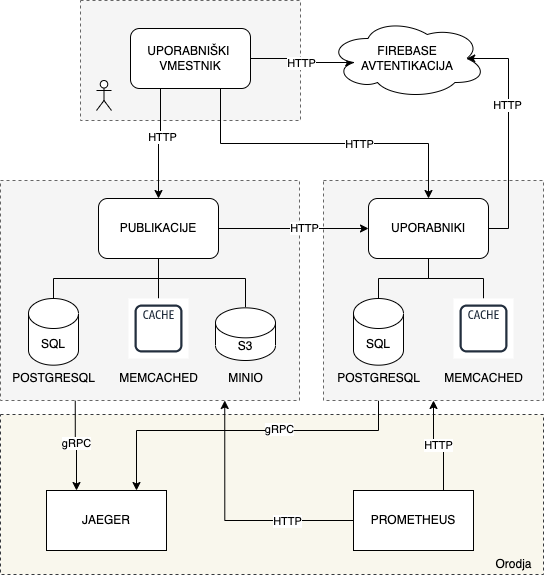
\includegraphics[width=0.75\textwidth]{slike/arch-done.png}
\end{center}
\caption{ Arhitektura projekta predstavljena z diagramom. }
\label{final-arch}
\end{figure}


% #####################################################################

% #####################################################################
\section{Zasnova projekta}
Arhitekturna zasnova močno vpliva na delovanje in razvoj aplikacije. Vsak arhitekturni koncept ima svoje prednosti in slabosti. Na projektu smo želeli predstaviti arhitekturo mikrostoritev. Ta vrsta arhitekture definira aplikacijo, sestavljeno iz majhnih samostojnih enot. Vsaka enota ima točno določeno funkcijo in lahko deluje neodvisno od ostalih enot.

V aplikaciji smo definirali dve mikrostoritvi (Slika \ref{app-architecture}). Ena storitev skrbi za delo s publikacijami, druga pa za delo z uporabniki. Storitvi med seboj komunicirata s protokolom \verb=HTTP=.

%% @ziga napaka v diagramu: "VMESTNIK" -> "VMESNIK"
\begin{figure}[h]
\begin{center}
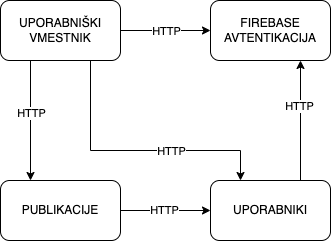
\includegraphics[width=0.5\textwidth]{slike/architecture.png}
\end{center}
\caption{ Arhitektura mikrostoritev naše aplikacije }
\label{app-architecture}
\end{figure}

% Z vpeljavo raznih vzorcev, smo definirali arhitekturni koncept, ki se izkaže kot dobra praksa. Uporabili smo vzorec repozitorija, s katerim smo ločili kodo, ki skrbi za pridobivanje in shranjevanje podatkov 

% Arhitekturni koncept kode sledi uporabi dobre prakse. Kodo, ki skrbi za pridobivanje in shranjevanje podatkov smo ločili 

Koncept kode sledi heksagonalni arhitekturi. Z omenjeno arhitekturo zagotovimo, da je domenska logika neodvisna od trenutne infrastrukture. Uporabljamo vzorec repozitorija s katerim ločimo poslovno kodo od kode, ki skrbi za pridobivanje in shranjevanje podatkov. Za vsako zbirko podatkov smo definirali vmesnik (ang. Interface). Vmesnik definira metode, ki so lahko različno implementirane glede na infrastrukturo. Ta način nam omogoča enostavno spreminjanje implementacije v primeru, ko hočemo zamenjati infrastrukturo podatkovne baze. 

Za potrebe aplikacije smo vmesnike implementirali s $PostgreSQL$ podatkovno baze (Koda \ref{lst:article-repository}). 
\begin{lstlisting}[language=go, style=mystyle,caption={Vmesnik, ki definira repozitorij za publikacije},label=lst:article-repository]
// ArticleRepository defines the datastore handling persisting Article records.
type ArticleRepository interface {
	Create(ctx context.Context, article *Article, callback ArticleCallbackFn) (*Article, error)
	Delete(ctx context.Context, id utils.BINARY16) error
	Find(ctx context.Context, id utils.BINARY16) (*Article, error)
	Update(ctx context.Context, article *Article, callback ArticleCallbackFn) (*Article, error)
}

// ArticleSearchRepository defines the datastore handling searching Article records.
type ArticleSearchRepository interface {
	Search(ctx context.Context, args SearchParams) (SearchResults, error)
}
\end{lstlisting}

% #####################################################################
\section{Komunikacija in dokumentacija}
Za komunikacijo z zalednim delom aplikacije uporabljamo protokol \verb=HTTP= (Hypertext Transfer Protocol). \verb=HTTP= je brezstanjski protokol aplikacijskega sloja, ki skrbi za komunikacijo med odjemalcem in strežnikom. Deluje po protokolu \verb=zahteva-odgovor= (angl. request–response ali request–reply) v modelu odjemalec-strežnik (Slika \ref{communication-flow}). Zahtevki se izvajajo sinhrono, kar pomeni, da je povezava med odjemalcem in strežnikom odprta toliko časa, dokler strežnik ne odgovori s podatki, oziroma do neke časovne omejitve \cite{http-rfc}. 


\begin{figure}[h]
\begin{center}
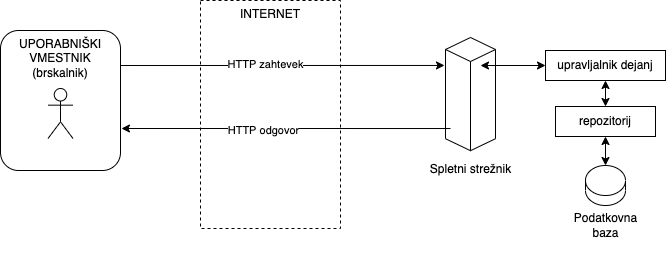
\includegraphics[width=0.9\textwidth]{slike/communication.png}
\end{center}
\caption{ Prikaz komunikacije po protokolu zahteva-odgovor }
\label{communication-flow}
\end{figure}

Za komunikacijo z zalednim delom aplikacije smo definirali aplikacijski programski vmesnik (API), z uporabo protokola HTTP. Vmesnik je arhitekturno predstavljen kot REST API, kar pomeni, da je vsak vir predstavljen kot spletna storitev z enoznačnim naslovom URL. Za pridobivanje in urejanje podatkov uporabljamo standardne metode HTTP: GET, POST, PUT, DELETE. Sistemi, ki uporabljajo REST pristop stremijo k hitri, odzivni in stabilni komunikaciji med odjemalcem in strežnikom.

Primer definiranih virov za pridobivanje, urejanje, brisanje in kreiranje publikacij v sistemu:
\begin{description}
   
\begin{itemize}
    \item \textbf{GET /articles/list} - Vrni seznam publikacij
    \item \textbf{POST /articles/add} - Shrani novo publikacijo
    \item \textbf{GET /articles/:uuid/get} - Vrni publikacijo za dodeljen ID 
    \item \textbf{DELETE /articles/:uuid/delete} - Izbriši publikacijo za dodeljen ID
    \item \textbf{PUT /articles/:uuid/update} - Osveži obstoječo publikacijo
    \item \textbf{POST /articles/:uuid/upload-files} - Pripni datoteko k publikaciji
    \item \textbf{DELETE /articles/:uuid/files/:file-uuid} - Odstrani datoteko publikacije
\end{itemize}
\end{description}

Pri definiranju komunikacijskega vmesnika smo sledili znanemu standardu \verb=OpenApi 3.0=. Ustvarili smo specifikacijske datoteke, kjer je definiran vsak klic, ki ga je mogoče izvesti na zaledni del. Te specifikacije nam pomagajo pri grajenju dokumentacije (Slika \ref{swagger-docs}), v našem primeru pa na podlagi API specifikacij tudi generiramo kodo, katera skrbi za komunikacijo med odjemalcem in strežnikom. Generirana koda je enostavna za uporabo in je postala dobra praksa saj s tem tudi zagotovimo, da je dokumentacija komunikacijskega vmesnika ves čas pravilna. 

\newpage
\begin{figure}[h]
\begin{center}
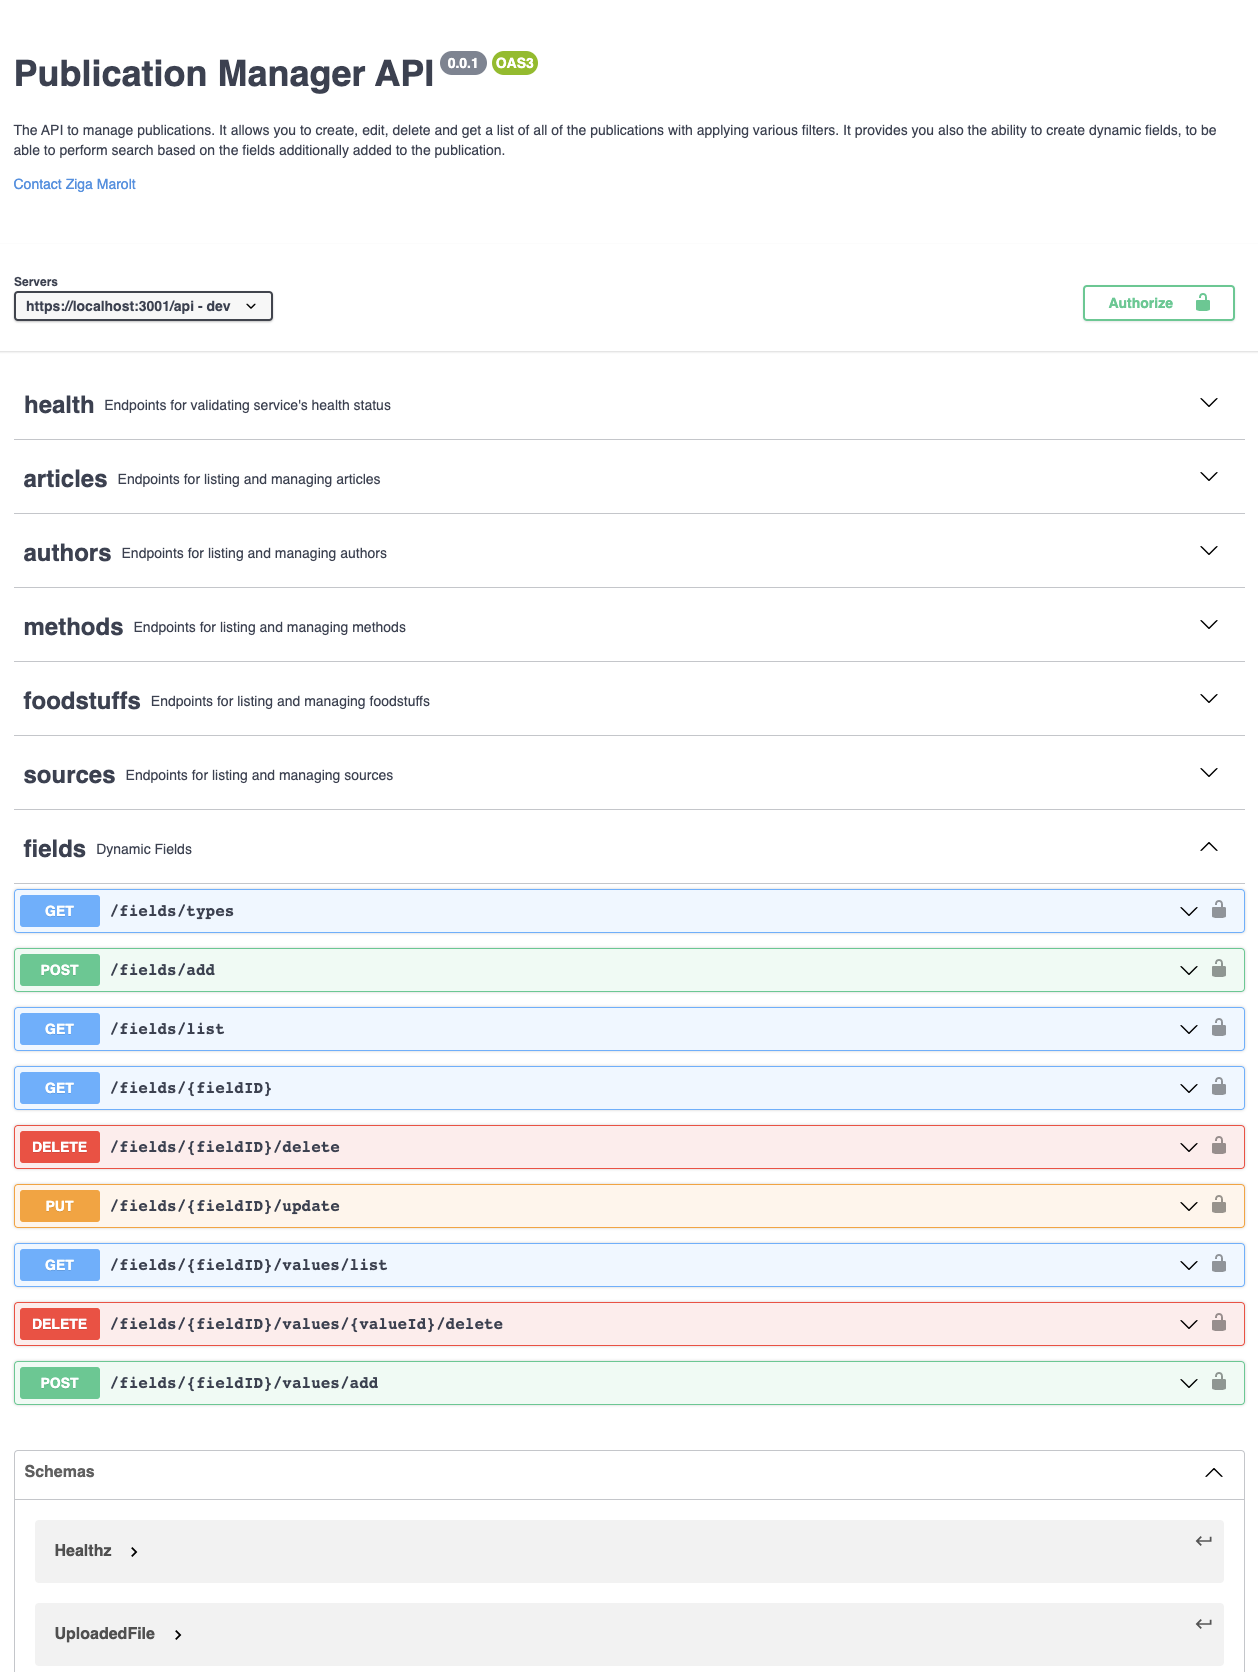
\includegraphics[width=1\textwidth]{slike/documentation.png}
\end{center}
\caption{ Dokumentacija z orodjem Swagger. }
\label{swagger-docs}
\end{figure}
\clearpage


Da je delo enostavno, smo naredili skripto, ki poskrbi da se generira željena koda odjemalca in strežnika (Koda \ref{lst:generator-script}).
\begin{lstlisting}[language=bash, style=mystyle, caption={Skripta, ki poskrbi za generiranje kode za posamezno storitev},label=lst:generator-script]
#!/bin/bash
set -e

readonly service="$1"

readonly docker_image="openapitools/openapi-generator-cli:v5.3.0"

docker run --rm --env "JAVA_OPTS=-Dlog.level=error" -v "${PWD}:/local" \
  "$docker_image" generate \
  -i "/local/api/openapi/$service.yml" \
  -g javascript \
  -o "/local/web/src/services/clients/$service"
\end{lstlisting}
    

\clearpage
Za zaledni del uporabimo generator \verb=Swagger=, s katerim pridobimo osnovno kodo za strežnik HTTP, ki posreduje podatke odjemalcem. Omogoča nam osnovno validacijo podatkov, ki so poslani v zahtevku in le-te pretvori v primerno strukturo, s katero je enostavno manipulirati dalje v aplikaciji. 

Za čelni del generiramo odjemalce JavaScript z \verb=OpenApi= generatorjem, ki poskrbijo za komunikacijo s strežnikom na zalednem delu. S tem nam ni potrebno skrbeti, da bi skonstruirali zahtevek v napačni obliki.


Za izmenjavo podatkov med odjemalcem in strežnikom uporabljamo strukturo JSON (angl. JavaScript Object Notation), ki je preprosta oblika za izmenjavo podatkov in je neodvisna od programskega jezika. Zaradi besedne zasnove je enostaven za branje in pisanje tako ljudem kot tudi računalnikom \cite{json-rfc}.

\begin{lstlisting}[language=bash, style=mystyle,caption={Primer izvedbe API klica in odgovora},label=lst:api-call-example]
 curl --request POST \
 --url https://localhost:3001/api/authors/{authorID}/update \
 --header 'Authorization: Bearer ==token==' \
 --header 'Content-Type: application/json' \
 --data '{
    "name": "John Doe"
 }'
\end{lstlisting}

Komunikacija je lahko uspešna ali ne, zato je potrebno odjemalcu odgovoriti z ustrezno kodo, kot je definirano v protokolu HTTP. Statuse lahko razdelimo v različne skupine, ki predstavljajo napake storjene na strani odjemalca (4xx), napake, storjene na strani strežnika (5xx) in uspešno obdelane zahtevke (2xx). V tabeli ~\ref{table:http-codes} so prikazane vse napake, ki jih aplikacija lahko vrne. 
\begin{table}[h]
\begin{tabular}{ll}
\textbf{Koda napake} & \textbf{Pomen}                                                    \\
200                  & $OK$ - Zahtevek je uspešno izveden                                  \\
400                  & $Bad Request$ - Zahtevek ni veljaven                                \\
401                  & $Unauthorized$ - Žeton ni veljaven                                  \\
403                  & $Forbidden$ - Ni zadostnih pravic                                   \\
404                  & $Not Found$ - Vir ne obstaja                                        \\
422                  & \begin{tabular}[c]{@{}l@{}}$Unprocessable Entity$ - Zahtevek vsebuje neveljavne \\ podatke \end{tabular}   \\
429                  & \begin{tabular}[c]{@{}l@{}}$Too Many Requests$ - Narejenih preveč zahtevkov v \\ časovnem obdobju\end{tabular} \\
500, 502, 503, 504   & $Internal Server Error$ - Napaka na zalednem sistemu
\end{tabular}
\caption{Seznam napak, ki jih vrača strežnik}
\label{table:http-codes}
\end{table}


\newpage
% #####################################################################
\section{Avtentikacija in avtorizacija}
Za preverjanje pristnosti uporabnika med posameznimi zahtevki uporabljamo žeton JWT (JSON Web Token), v katerem je zapisan identifikator uporabnika in njegova vloga. Žeton je brezstanjski, kar pomeni, da ni nikjer shranjen. To nam omogoča izdelavo ločenih sistemov, ki niso vezani na določeno shemo preverjanja pristnosti. Žeton je lahko ustvarjen kjer koli in porabljen v katerem koli sistemu, ki za podpis žetona uporablja isti skrivni ključ (ang. secret key). Tako nam podatkov o uporabniku ni potrebno vedno znova, ob vsakem zahtevku preveriti s podatki v bazi.

Odjemalec v glavi zahtevka pošlje \verb=Bearer= žeton s katerim identificira uporabnika. Ker ima žeton določeno življenjsko dobo, je bilo potrebno poskrbeti tudi za osveževanje tega žetona (Slika \ref{token-flow}). Ob vsaki spremembi žetona odjemalec nastavi novo vrednost v glavi zahtevka. S tem poskrbimo, da je žeton ves čas delujoč in veljaven (Koda \ref{lst:auth-set-token}).

\begin{figure}[h]
\begin{center}
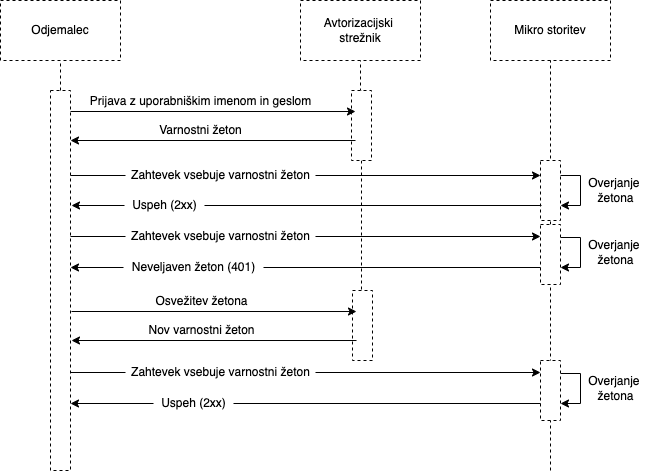
\includegraphics[width=0.9\textwidth]{slike/token-flow.png}
\end{center}
\caption{ Diagram prikazuje komunikacijo z uporabo žetona (JWT) }
\label{token-flow}
\end{figure}

Strežnik, ki žeton prebere na podlagi skrivnega ključa, preveri, če je žeton veljaven. Uporabljen skrivni ključ je enak kot ključ s katerim je bil žeton ustvarjen. S tem zagotovimo, da se podatki vmes niso spremenili.

V zalednem sistemu se ob vsakem zahtevku sproži akcija za overjanje. Napisali smo funkcijo poznano kot \verb=middleware= (Koda \ref{lst:auth-middleware}), ki na podlagi skrivnega ključa preveri, če je žeton veljaven. Uporabljen skrivni ključ je enak kot ključ s katerim je bil žeton ustvarjen. S tem zagotovimo, da se podatki vmes niso spremenili. V primeru, da žeton ni veljaven, odgovorimo z ustreznim odgovorom \verb=401 - Unauthorized=. 
%% @ziga tukaj se ti del besedila ponavlja

\begin{lstlisting}[style=mystyle,caption={Izsek kode za nastavljanje žetona posameznemu odjemalcu},label=lst:auth-set-token]
export function setApiClientsAuth(idToken) {
    users.authentications.bearerAuth.accessToken = idToken;
    fields.authentications.bearerAuth.accessToken = idToken;
    ...
}
\end{lstlisting}

V primeru, da je žeton veljaven, preberemo vrednost žetona, ki vsebuje identifikator uporabnika, uporabniško ime, elektronski naslov in vlogo (ang. role) uporabnika. S prebranimi vrednostmi kreiramo objekt uporabnika in nadaljujemo s procesiranjem zahtevka.

  \begin{lstlisting}[language=go,style=mystyle,caption={Izsek kode za preverjanje pristnosti uporabnika},label=lst:auth-middleware]
func UserMiddleware(ctx context.Context, authService Service) MiddlewareFunc {
	return func(authToken string) (*User, error) {
			if !strings.HasPrefix(authToken, "Bearer ") {
			return nil, apierrors.Forbidden()
		}

		authToken = strings.TrimSpace(strings.Replace(authToken, "Bearer", "", 1))
		if authToken == "" {
			return nil, apierrors.Unauthorized()
		}

		token, err := authService.VerifyToken(ctx, authToken)
		if err != nil {
			return nil, apierrors.Unauthorized()
		}
		
		return &User{
			UID:         UID(token.UID),
			Email:       token.Claims["email"].(string),
			Role:        token.Claims["role"].(string),
			DisplayName: token.Claims["name"].(string),
		}, nil
	}
}
\end{lstlisting}

Preverjanje pravic se preveri v kodi, ki vsebuje logiko, kaj naj se zgodi z zahtevkom (Koda \ref{lst:auth-check-role}). Najprej preverimo, če je zahtevek od uporabnika, ki ima zadostne pravice za izvajanje tega zahtevka. V primeru, da uporabnik nima zadostnih pravic, mu odgovorimo z odgovorom \verb=403 - Forbidden=. Če uporabnik pravice ima, se procesiranje zahtevka nadaljuje.

\clearpage
\begin{lstlisting}[language=go,style=mystyle,caption={Izsek kode za preverjanje pravic uporabnika},label=lst:auth-check-role]
// DeleteUserHandler handles the delete user request
func (h *HttpHandler) DeleteUserHandler() users.DeleteUserHandlerFunc {
	return func(params users.DeleteUserParams, user *auth.User) middleware.Responder {

		// check if user has rights to perform this action
		if user.Role != string(domain.AdminRole) {
			return users.NewDeleteUserHandlerForbidden()
		}

		uuid, err := utils.StringToBinary16(string(params.UserID))
		if err != nil {
			return h.returnError(err)
		}
		u, err := h.app.Commands.DeleteUser.Handle(params.HTTPRequest.Context(), command.DeleteParamsCmd{
			UserUUID: uuid,
		})

		if err != nil {
			return h.returnError(err)
		}

		return users.NewUpdateUserNoContent()
	}
}
\end{lstlisting}
\clearpage
\section{Podatkovna baza }

% #####################################################################
\subsubsection{Upravljanje s podatkovno shemo}
Postavitev podatkovne sheme se izvede v zbirki podatkov vsakič, ko je potrebno posodobiti ali povrniti shemo baze podatkov na novo ali na starejšo različico. Ta proces imenujemo tudi migracija podatkovne sheme.

V aplikaciji uporabljamo programsko orodje \verb=go-migrate=. Omogoča izvajanje migracij za različne vrste podatkovnih baz, med njimi tudi PostgreSQL, katero uporabljamo mi. Z orodjem ustvarimo migracijske datoteke, v katere napišemo shemo podatkovne baze. Vsaka migracijska akcija vsebuje dve datoteki. V eni datoteki so definirani ukazi (SQL stavki) za postavitev podatkovne sheme (Koda \ref{lst:schema-migration}), in v drugi ukazi za  povrnitev podatkovne sheme v stanje pred migracijo.


\begin{lstlisting}[language=sql, style=mystyle,caption={Izsek koda, za kreiranje tabele "articles", namenjeno hranjenju podatkov o publikacijah.},label=lst:schema-migration]
-- Table Definition
CREATE TABLE "articles"
(
    "uuid"            uuid      NOT NULL PRIMARY KEY,
    "source_uuid"     uuid      NOT NULL REFERENCES sources (uuid) ON DELETE CASCADE,
    "title"           text      NOT NULL,
    "url"             text      NOT NULL DEFAULT '',
    "year"            int,
    "comment"         text      NOT NULL DEFAULT '',
    "temperature_min" int       NOT NULL DEFAULT 0,
    "temperature_max" int       NOT NULL DEFAULT 0,
    "file_uuid"       uuid,
    "approved_by"     uuid,
    "released_at"     timestamp          DEFAULT null,
    "created_at"      timestamp NOT NULL DEFAULT now(),
    "updated_at"      timestamp NOT NULL DEFAULT now()
);
\end{lstlisting}

% #####################################################################
\subsubsection{ Struktura podatkov }
Z migracijami smo definirali celotno strukturo podatkovne baze, ki jo potrebujemo. Definirali smo 13 tabel, ki skrbijo, da so podatki pravilno shranjeni. Vizualni prikaz tabel in medsebojnih relacij je viden na sliki ~\ref{database-diagram-er}. Opis posameznih tabel:
\begin{description}
\item[gomigrate]: Tabela vsebuje informacije o stanju migracij. Ob vsakem izvajanju migracij se v tabelo zapiše identifikator migracije, glede na katerega se izvajajo nadaljnje migracije za podatkovno shemo. 

\item[users]: Tabela vsebuje informacije o uporabnikih, ki so registrirani v sistem. Uporabniki se v aplikaciji razlikujejo glede na enoličen identifikator UUID in unikaten e-poštni naslov (``email``). 

\item[articles]: Tabela vsebuje informacije o publikacijah, vnesenih s strani uporabnika. Vsebuje informacije, kot so naslov, leto izdaje, komentar, najvišja in najnižja temperatura. Poleg informacij, ki jih vnese uporabnik, imamo tudi evidenco o tem, kdo je potrdil publikacijo. Tabela vsebuje tudi relacije z ostalimi entitetami, za povezavo z metodami, avtorji, viri, dinamičnimi podatki in živili. Ena publikacija lahko ima le en vir, zato je ta relacija definirana s tujim ključem v isti tabeli, prav tako velja za pripeto datoteko. 

Ostale relacije, kot so živila, pa so definirana kot mnogo-proti-mnogo, kar pomeni, da potrebujemo medsebojne tabele za povezovanje entitet.
\begin{itemize}
    \item article\_methods: tabela za povezovanje publikacij in metod
    \item article\_foodstuffs: tabela za povezovanje živil in publikacij
    \item article\_authors: tabela za povezavo publikacij in avtorjev
    \item article\_fields: tabela za povezavo dinamičnih podatkov s publikacijami
\end{itemize}

\item[authors]: Tabela vsebuje informacije o avtorjih, katerih publikacije so vnesene v naši aplikaciji. Za povezavo se uporablja medsebojna tabela $article\_authors$.

\item[methods]: Tabela vsebuje informacije o metodah, ki jih posamezne publikacije uporabljajo. Za povezavo se uporablja medsebojna tabela $article\_methods$.

\item[foodstuffs]: Tabela vsebuje informacije o živilih, ki so bila uporabljena pri posameznih publikacijah. Za povezavo se uporablja medsebojna tabela $article\_foodstuffs$.

\item[foodstuffs]: Tabela vsebuje informacije o živilih, ki so registrirani v sistem. Za povezavo se uporablja medsebojna tabela $article\_foodstuffs$.

\item[sources]: Tabela vsebuje informacije o virih, iz katerih črpamo publikacije. Tip vira je definiran kot $enum$, čigar vrednost je definirana kot "knjiga", "internetni vir", "revija". Za definicijo tipa smo uporabili PostgreSQL ukaz:
\begin{lstlisting}[language=sql, style=mystyle]
CREATE TYPE source_type AS ENUM ('web','book','magazine')
\end{lstlisting}

\item[fields]: Tabela vsebuje informacije o vseh dinamično definiranih podatkih v aplikaciji. Podatki se razlikujejo glede na tip. Vsebujejo lahko enega ali več vrednosti. V primeru, da je podatek sestavljen iz večih vrednosti, uporabimo relacijsko tabelo $field\_values$, kjer so zapisane vrednosti za posamezen podatek.

\item[article\_fields]: Tabela vsebuje relacijo med dinamičnimi podatki in njihovimi vrednostmi. Za potrebe optimalnega iskanja hrani različne tipe vrednosti: 
\begin{itemize}
    \item value\_varchar: hrani tekstovno vrednost 
    \item value\_date: hrani časovno vrednost
    \item value\_number: hrani numerično vrednost
\end{itemize}
\end{description}

\subsubsection{Shranjevanje podatkov}
Potrebno je poskrbeti, da so podatki shranjeni v popolni obliki. V primeru, da pri shranjevanju pride do napake, jo je potrebno ustrezno rešiti. Da so podatki shranjeni v popolni obliki, uporabljamo transakcije. Transakcija je atomična enota, s čimer zagotovimo, da so vse poizvedbe izvedene uspešno. V primeru, da ena poizvedba ni bila uspešno izvedena, se vse poizvedbe, storjene v isti transakciji, povrnejo v stanje pred izvedbo. 

Posamezna metoda v repozitoriju poleg ostalih parametrov prejme še funkcijo, katera se izvede znotraj transakcije (Koda \ref{lst:transaction-call}). V primeru, da funkcija vrne napako, se transakcija resetira in povrne podatkovno bazo v stanje pred shranjevanjem.

\begin{lstlisting}[language=go,style=mystyle,caption={ Prikaz shranjevanja publikacije },label=lst:transaction-call]
func (h AddArticleHandler) Handle(ctx context.Context, cmd AddArticleParamsCmd) (res *domain.Article, err error) {
	res, err = h.repo.Create(ctx, article, func(ctx context.Context, a *domain.Article) error {
		return h.repo.AssignAuthors(ctx, a, cmd.Authors, func(ctx context.Context, a *domain.Article) error {
			return h.repo.AssignFoodstuffs(ctx, a, cmd.Foodstuffs, func(ctx context.Context, a *domain.Article) error {
				return h.repo.AssignMethods(ctx, a, cmd.Methods, func(ctx context.Context, a *domain.Article) error {
					return h.repo.AddExtraFields(ctx, a, fields)
				})
			})
		})
	})
	
	if err != nil {
		return res, errors.WrapErrorf(err, errors.ErrorCodeUnknown, "AddArticleHandler.repo")
	}
	
	return res, nil
}
\end{lstlisting}

Datotek, pripetih k publikacijam, ne shranjujemo v relacijsko podatkovno bazo. Definirali smo vmesnik, ki nam pove, katere metode moramo implementirati za pravilno delovanje (Koda \ref{lst:file-interface}). Implementirali smo repozitorij, ki uporablja S3 kompatibilnega odjemalca. Za hrambo teh datotek uporabljamo storitev Minio (\ref{minio-what}).

\begin{lstlisting}[language=go,style=mystyle,caption={Prikaz vmesnika za shranjevanje in branje datotek},label=lst:file-interface]
// FileRepository provides functions to uplaod and read file
FileRepository interface {
	UploadFile(ctx context.Context, rc io.ReadCloser, size int64) (*utils.BINARY16, error)
	GetFile(ctx context.Context, uuid utils.BINARY16) (io.ReadCloser, error)
}
\end{lstlisting}


\begin{figure}[ht]
\begin{center}
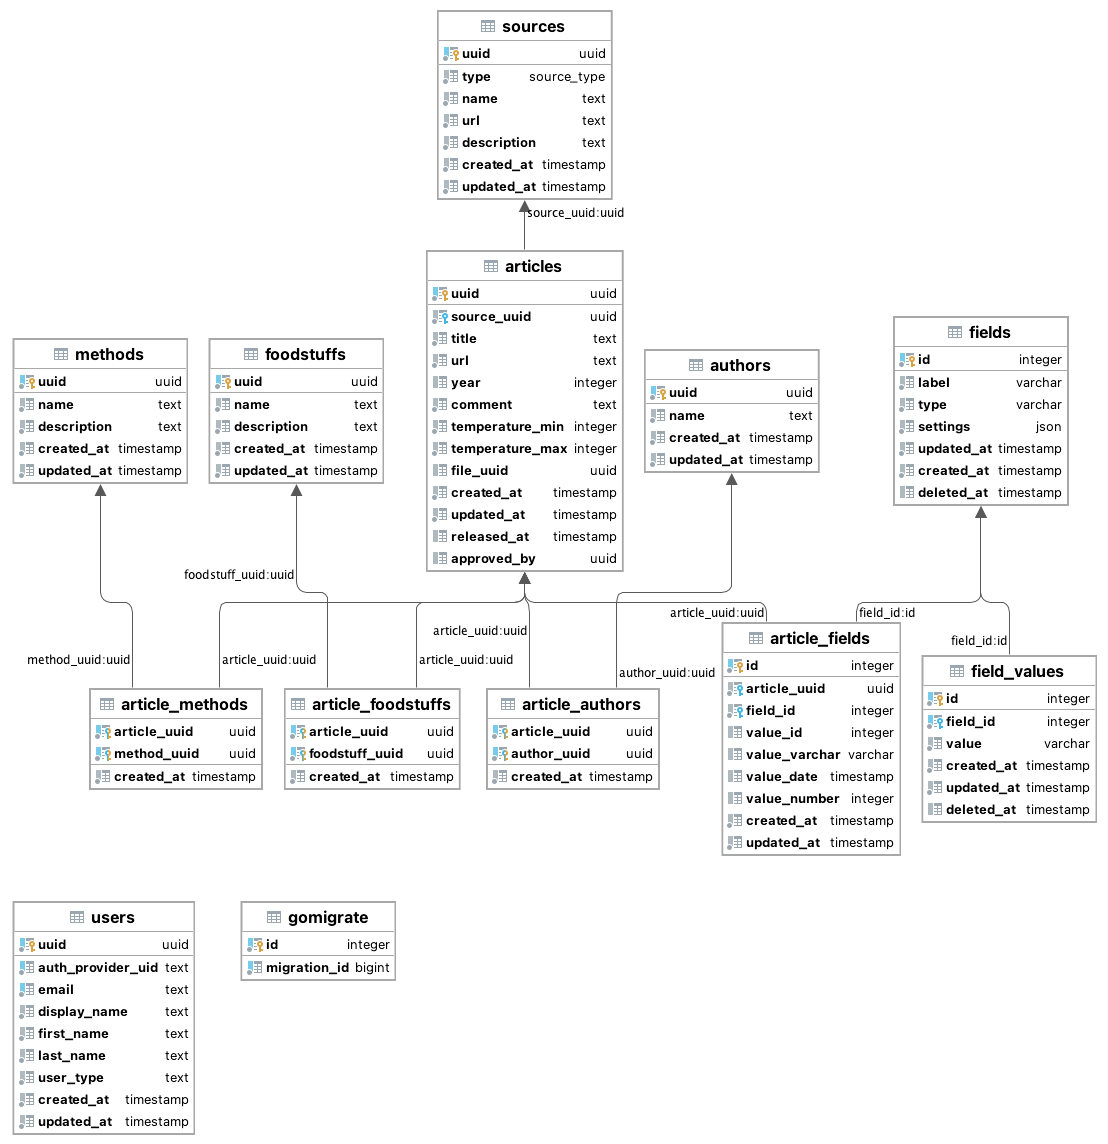
\includegraphics[width=1\textwidth]{slike/database-structure.png}
\end{center}
\caption{ Predstavitev podatkovne sheme z ER diagramom }
\label{database-diagram-er}
\end{figure}

% #####################################################################
\subsubsection{Branje podatkov}
V aplikaciji smo poskrbeli, da do težave z izvajanjem poizvedb po nepotrebnem ne bo prišlo. Pri poizvedovanju podatkov o publikacijah iz podatkovne baze je potrebno biti pozoren na število izvedenih klicev. Če nismo pazljivi, lahko pridemo do težave s poizvedbo \verb=n+1=. Ta se zgodi, ko del aplikacije izvede \verb=n= dodatnih poizvedb, da bi pridobil iste podatke, ki bi jih bilo mogoče pridobiti pri izvajanju primarne poizvedbe SQL. Večja kot je vrednost \verb=n=, več poizvedb bo izvedenih, večji je vpliv na zmogljivost. 

\clearpage
% #####################################################################
\section{Čelni del aplikacije}
Čelni del aplikacije uporablja ogrodje \verb=Vue.js= (\ref{vue-js-section}). Je zelo enostavno \verb=JavaScript= ogrodje s številnimi orodji in knjižnicami, s katerimi si poenostavimo in pohitrimo razvoj. Knjižnice, ki jih aplikacija potrebuje, so navedene v datoteki \verb=package.js= (Koda \ref{lst:pkg-snippet}). V omenjeni datoteki so navedeni tudi ukazi, s katerimi prožimo določene akcije, kot so gradnja statičnih paketov, postavitev spletnega strežnika za streženje datotek in gradnja CSS datotek s pomočjo knjižnice \verb=tailwind=. Za nadzor nad uporabljenimi knjižnicami skrbi orodje \verb=NPM= (angl. Node Package Manager).

\begin{lstlisting}[language=php, style=mystyle,caption={Izsek naštetih knjižnic in ukazov v datoteki package.json},label=lst:pkg-snippet]
{
  "name": "diploma",
  "version": "1.0.0",
  "private": true,
  "scripts": {
    "serve": "vue-cli-service serve",
    "build:tailwind": "npx tailwindcss ...",
  },
  "dependencies": {
    "@fortawesome/fontawesome-free": "^5.15.4",
    "@tailwindcss/forms": "^0.3.4",
    "@vueform/multiselect": "^2.2.1",
    "@vueform/slider": "^2.0.8",
    "core-js": "^3.19.1",
    "firebase": "^9.3.0",
    "jsonwebtoken": "^8.5.1",
    "litepie-datepicker": "^1.0.14",
    "lodash": "^4.17.21",
    "moment-timezone": "^0.5.34",
    "superagent": "^6.1.0",
    "v-tooltip": "^4.0.0-beta.2",
    "vue": "^3.2.21",
    "vue-router": "^4.0.0-0",
    "vue-toast-notification": "^2.0.1"
  },
  "devDependencies": {
     ...
    "sass": "^1.32.5",
    "sass-loader": "^10.1.1",
    "tailwindcss": "^2.2.19"
  }
}

\end{lstlisting}

% V tem delu bomo spoznali kako je zasnovan čelni del naše aplikacije in kako komunicira z zalednim sistemom. Pri razvoju tega dela aplikacije je potrebno biti pozoren na kar nekaj stvari, kot je naprimer zasnova na videz lepega, vendar uporabnega grafičnega vmestnika, preko katerega uporabnik varno komunicira z našim zalednim sistemom. Med samo uporabo in komunikacijo ne smemo pozabiti na ustrezno prikazovanje napak uporabniku, da sam uporabnik ve kdaj je do napake prišlo in kako jo odpraviti.


Ogrodje je odvisno od \verb=node.js= programskih datotek, zatorej moramo v sliko vsebnika namestiti potrebne stvari za delovanje tega ogrodja. Uporabimo obstoječo sliko vsebnika \texttt{node:17.3.0-alpine3.14}, ki že ima nameščena orodja kot so \texttt{node.js} in upravljalec paketkov \texttt{npm}. Ker je vsebnik uporabljen v razvojnem okolju, definiramo vrednost \texttt{NODE\_ENV} na vrednost \texttt{development}. Skripta \texttt{run.sh} je skopirana v sliko z dodatnimi pravicami za zagon. Na koncu se skipto sproži v izvajanje (Koda \ref{lst:dcf-node}).

\begin{lstlisting}[,style=mystyle,caption={Dockerfile datoteka za razvijanje Vue aplikacije},label=lst:dcf-node]
FROM node:17.3.0-alpine3.14

ENV NODE_ENV development

ADD start.sh /
RUN chmod +x /start.sh

CMD ["/run.sh"]
\end{lstlisting}

V datoteki $start.sh$ (Koda \ref{lst:dcf-run}) so navedeni ukazi, ki se zgodijo ob vsakem zagonu vsebnika. Ukaz \texttt{npm install} namesti vse potrebne knjižnice, ki jih v aplikaciji uporabljamo. Ukaz \texttt{npm serve} pa zažene spletni strežnik, ki streže vsebino aplikacije iz trenutnega direktorija.

\begin{lstlisting}[language=bash,style=mystyle,caption={Ukazna datoteka, ki naloži potrebne knjižnice in streže aplikacijo},label=lst:dcf-run]
set -e

npm install
npm serve
\end{lstlisting}

Pomembno je tudi poudariti, da je aplikacija enostranska (angl. single-page), kar pomeni, da deluje znotraj brskalnika in ne potrebuje ponovnega nalaganja strani med svojim delovanjem. Je le ena sama stran, ki jo obiščemo in na kateri se nato naloži vso ostalo vsebino s pomočjo kode JavaScripta.

Kot je razvidno iz prikaza zagnanih vsebnikov (Koda: \ref{lst:running-containers}), ima čelni del odprta vrata 80, kar pomeni, da je stran dostopna na lokalnem spletnem naslovu \url{http://localhost:80/}. 

% #####################################################################
\section{Razvoj vnosa dinamičnih podatkov}
Za potrebe aplikacije smo razvili popolnoma dinamičen način za dodajanje novih parametrov publikacije. Te paremetre lahko dodajamo, urejamo in brišemo tudi med tem, ko urejamo publikacijo, in kasneje izvajamo razne filtre nad vnesenimi podatki.

\begin{figure}[h]
\begin{center}
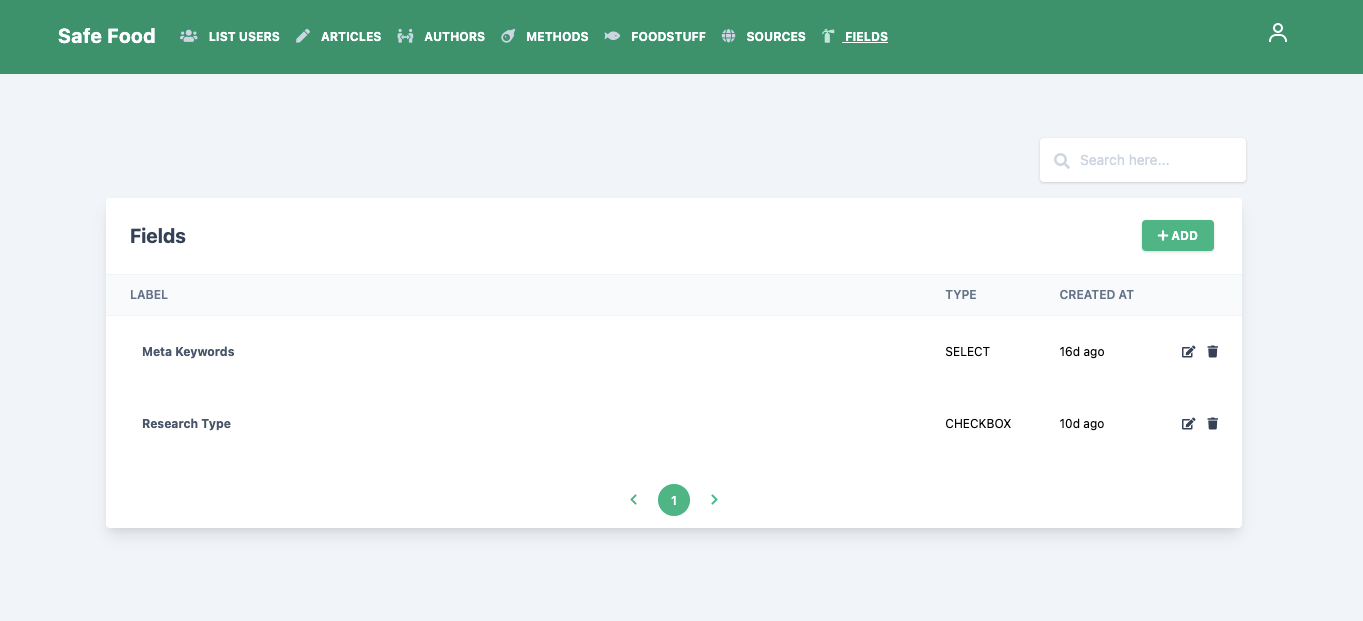
\includegraphics[width=1\textwidth]{slike/fields-list.png}
\end{center}
\caption{ Stran za prikaz in urejanje dinamičnih parametrov. }
\label{fields-list}
\end{figure}

Zaradi potrebe po razlikovanju po različnih tipih podatkov smo definirali več podatkovnih tipov, ki predstavljajo posamezne podatke. Zaradi raznolikosti med podatki vseh podatkov ne moremo predstaviti enako. Podatek, predstavljen kot številka, se ne odraža enako kot podatek, ki je predstavljen kot tekstovno polje. Katere tipe podatkov aplikacija podpira, je definirano v zalednem sistemu in je dostopno preko aplikacijskega programskega vmesnika (Koda \ref{lst:supported-fields}). 

\begin{figure}[h]
    \centering
    \begin{lstlisting}[language=bash, style=mystyle,caption={Izsek aplikacijskega vmesnika za pridobitev vseh podprtih podatkovnih tipov v aplikaciji},label=lst:supported-fields]
curl --request GET \
  --url https://localhost:3001/api/fields/types \
  --header 'Authorization: Bearer ==token==' \
  --header 'Content-Type: application/json'
{
  "types": [
    {
      "name": "select",
      "has_values": true,
      "settings": [
        {
          "name": "string",
          "type": "number",
          "default_value": "string"
        }
      ]
    }
  ]
}
\end{lstlisting}
\end{figure}

% \begin{figure}[h]
% \begin{center}
% 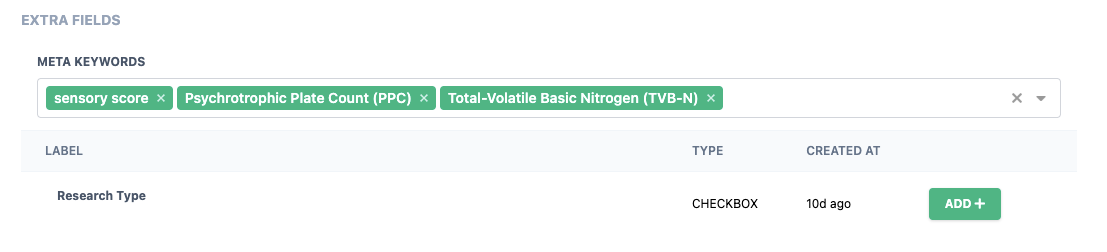
\includegraphics[width=1\textwidth]{slike/select_example_usage.png}
% \end{center}
% \caption{ Prikaz uporabe dinamično definiranega parametra, tipa select, z možnostjo izbere enega ali več podatkov. }
% \label{field-usage-example-select}
% \end{figure}


% % #####################################################################
% \subsection{Tipi podatkov}

% #####################################################################
\subsubsection{Vnosno polje}
Vnosno polje predstavlja podatek, ki ga je potrebno vnesti vsakič znova in nima definirane nobene vnaprej določene vrednosti. Vnosno polje je lahko predstavljeno kot številčna vrednost, ali pa kot tekstovno polje. 
Za ta podatek imamo možnost vnosa mnogih vrednosti, tako da definiramo podatek kot ponavljajoč podatek - \verb=repeatable=. To je uporabno za primere, ko hočemo dodati zraven publikacije enega ali več spletnih virov.

\begin{figure}[h]
\begin{center}
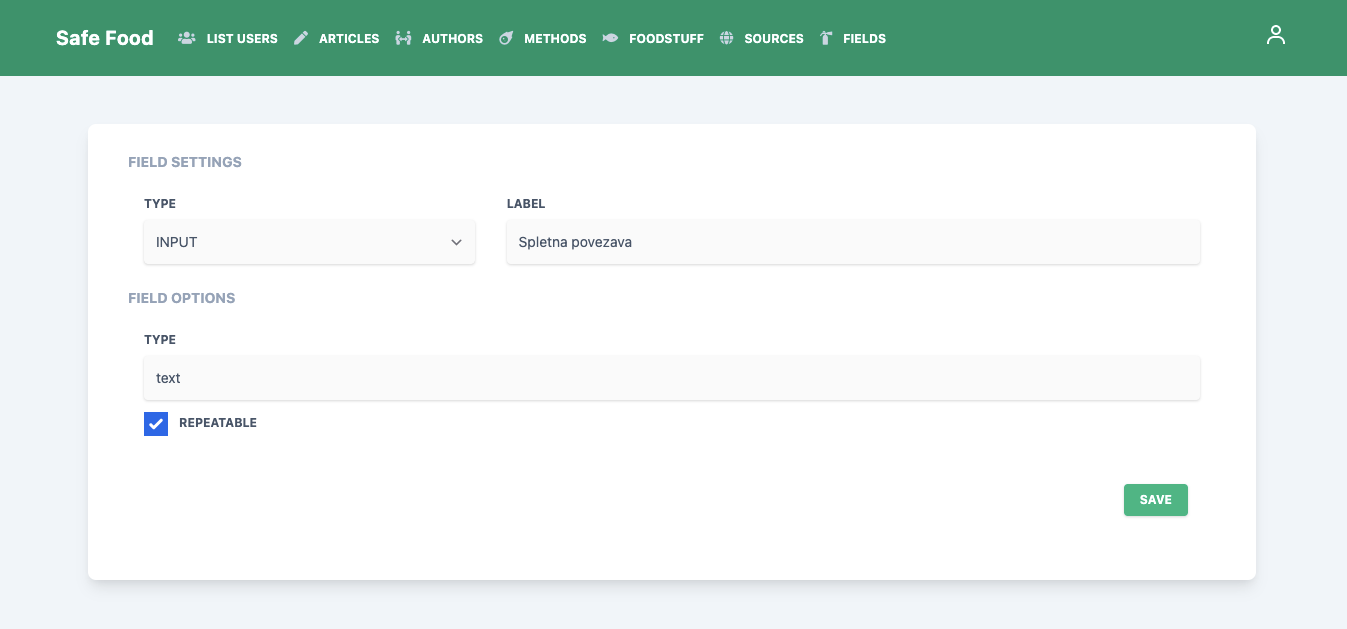
\includegraphics[width=1\textwidth]{slike/type_input.png}
\end{center}
\caption{ Definiranje vnosnega polja tipa $input$. }
\label{type-input}
\end{figure}

Na sliki \ref{type-input} je razvidno, kako se definira podatek imenovan \sn{Spletna povezava}. Vrednost spletne povezava je tekstovnega tipa, zato smo za vrednost izbrali \verb=text=. Izbrali smo tudi vrednost \verb=repeatable=, ker želimo omogočiti več vnosov spletnih povezav. Dodan parameter se lahko pojavi in je na voljo med urejanjem publikacije. 

Na dnu se nam prikaže vnosno polje, za katerega lahko izberemo in definiramo njegovo vrednost (Slika \ref{fields-usage}). Ker je parameter definiran tako, da je lahko predstavljen z več kot eno vrednostjo, se nam ponudi gumb za dodajanje nove vrednosti.

% #####################################################################
\subsubsection{Izbirno polje - Select}
\label{type-select-page}
Ta podatek predstavlja podobne vrednosti, kot vnosno polje \sn{Input}, z razliko, da so vrednosti lahko že vnaprej definirane. Te vrednosti nam omogočajo hitrejše vnašanje podatkov. Na voljo je tudi iskanje po vnesenih vrednostih in sprotno dodajanje vrednosti v primeru, da vrednost še ne obstaja. Vse to je možno nastaviti med samim definiranjem parametra (Slika \ref{type-select}). Na voljo je tudi možnost izbire več kot ene vrednosti, z izbiro opcije \verb=multiple=.

\begin{description}
\item[Opis posameznih opcij, med samim definiranjem parametra]:
	\begin{itemize}
		\item \textbf{taggable} - omogoča dodajanje novih vrednosti med samim urejanjem
		\item \textbf{multiple} - omogoča izbiro več kot ene vrednosti
		\item \textbf{searchable} - omogoča iskanje po vnesenih vrednostih
	\end{itemize}
\end{description}

\begin{figure}[h]
\begin{center}
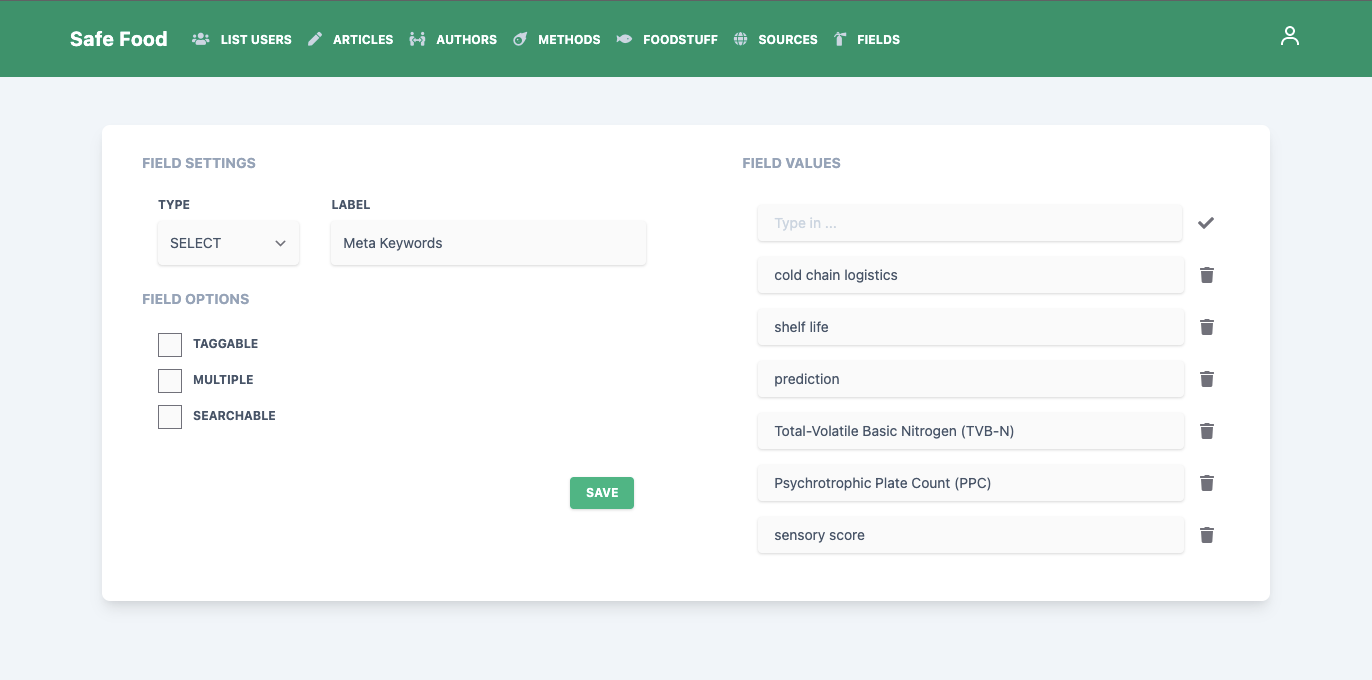
\includegraphics[width=1\textwidth]{slike/type_select.png}
\end{center}
\caption{ Definiranje vnosnega polja tipa $select$. }
\label{type-select}
\end{figure}


% #####################################################################
\subsubsection{Izbirno polje - checkbox}
\label{type-checkbox-page}
Ta predstavlja podatek, katere vrednosti so statične in vnaprej definirane. Vnos podatkov je podoben kot pri \sn{izbirnem polju - Select} (Slika \ref{type-select-page}), z razliko, da je podatek prikazan na drugačen način. Ta tip podatka nam ne omogoča iskanja po vrednostih in sprotnega dodajanja med samim urejanjem publikacije.

\begin{figure}[h]
\begin{center}
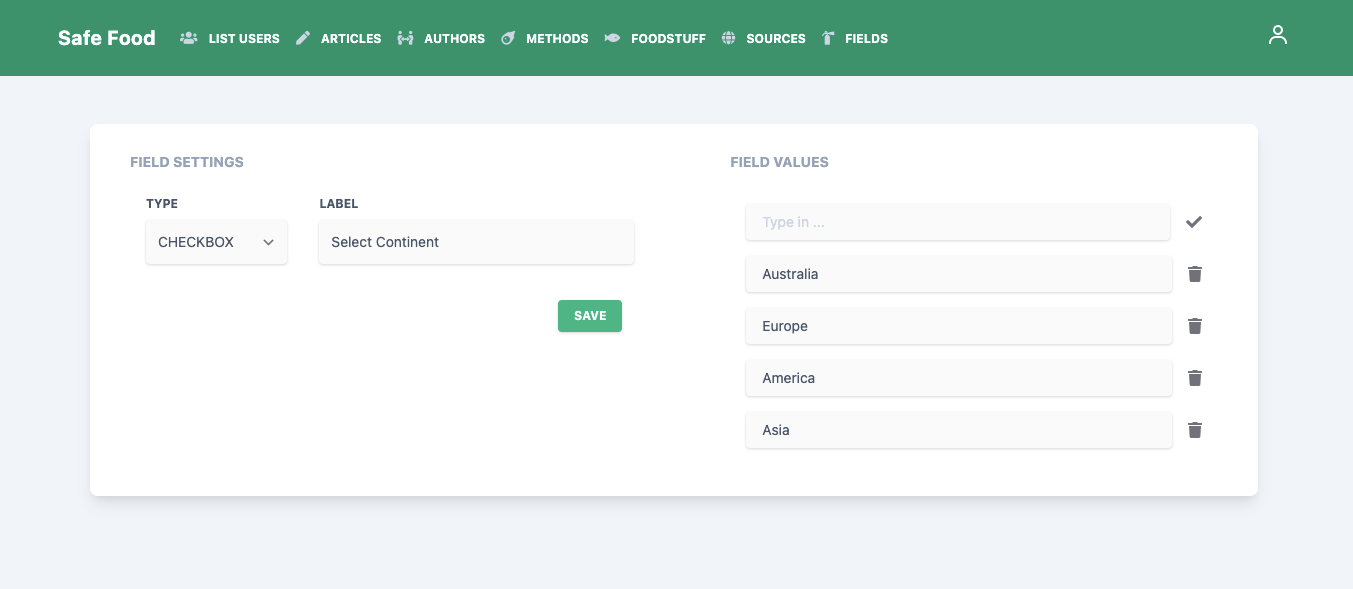
\includegraphics[width=1\textwidth]{slike/type_checkbox.png}
\end{center}
\caption{ Definiranje vnosnega polja tipa $checkbox$. }
\label{type-checkbox}
\end{figure}

% #####################################################################
\subsubsection{Polje za izbiranje časovnega podatka (datum)}
Predstavlja podatek, ki ima časovno vrednost. Uporabniku je omogočeno definiranje podatka z izbiro datuma in časa na koledarju (Slika \ref{type-date}). 

Uporabili smo minimalistično knjižnico \verb=Day.js=, ki z enostavnim aplikacijskim vmesnikom razčlenjuje, preverja, manipulira in prikazuje datume in ure za sodobne brskalnike. Ponuja tudi podporo z ostalimi knjižnicami, kot je na primer bolj priznana knjižnica \verb=Moment.js=.


\begin{figure}[h]
\begin{center}
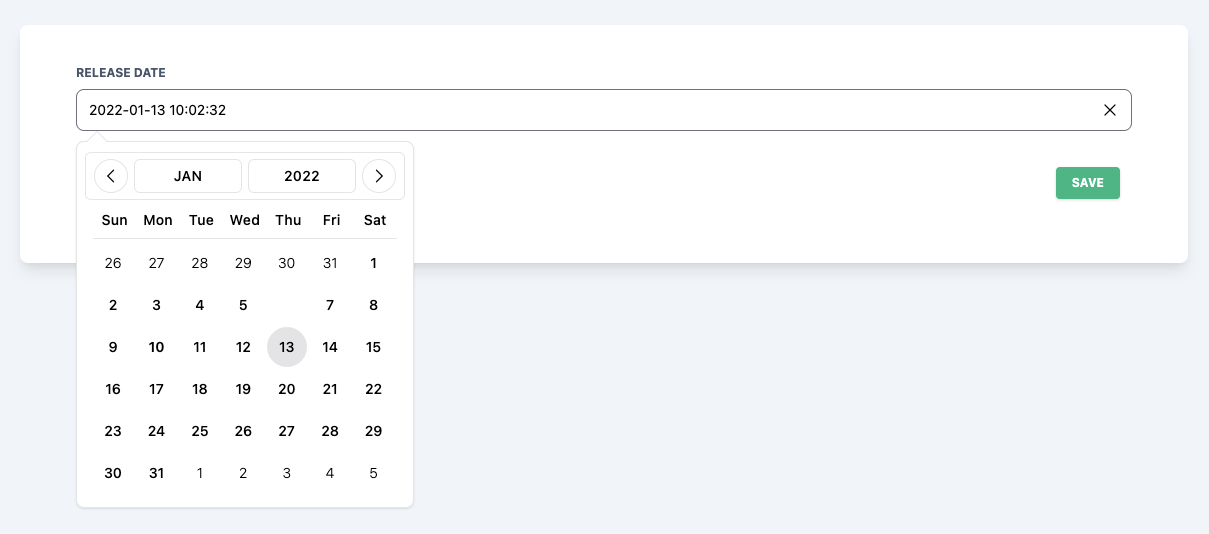
\includegraphics[width=1\textwidth]{slike/type_date.png}
\end{center}
\caption{ Prikaz grafičnega vmesnika za izbiranje datuma. }
\label{type-date}
\end{figure}
% #####################################################################

\subsubsection{Nalaganje datoteke}
Ta komponenta nam omogoča nalaganje datoteke za posamezno publikacijo. Na voljo je dodajanje slik in datotek tipa \verb=.pdf=. Ostalih vrst datotek aplikacija ne sprejme.
% #####################################################################

% +++++++++++++++++++++++++++++++++++++++++++++
% ++++++++ PREDSTAVITEV APLIKACIJE ++++++++++++
% +++++++++++++++++++++++++++++++++++++++++++++
\chapter{Predstavitev aplikacije}
% V prejšnjih poglavjih smo spoznali terminologijo, tehnologije in implementacijo teh tehnologij v našo aplikacijo. V tem poglavju pa bomo spoznali uporabo aplikacije, ki smo jo izdelali.

Aplikacija, ki smo jo poimenovali \sn{Safe Food} je sestavljena iz zalednega in čelnega dela. Zaledni del vključuje več komponent, ki sledijo arhitekturni postavitvi mikrostoritev. Čelni del pa je enostavna aplikacija, napisana v programskem ogrodju \verb=Vue.js=. Namenjena je uporabniku, zato je pomembno, da je na videz enostavna in pregledna, hkrati pa tudi hitra in funkcionalna. 


% #####################################################################
\section{Uvodna stran}
\label{landing-page}
Ob obisku spletnega mesta \url{http://localhost} se odpre \sn{Uvodna stran} (Slika \ref{landing-page}). Stran omogoča lokalno uporabo aplikacije in povezave na zunanje vire, kjer lahko pridobimo koristne informacije o živilih. Spodaj je povezava do strani Univerze v Ljubljani in pa do prijave oziroma registracije v aplikacijo.

S klikom na gumb \sn{Vstopi v aplikacijo}, nadaljujemo v aplikacijo. V primeru, da smo v aplikaciji že prijavljeni, se nam prikaže stran z urejenimi publikacijami, nad katerimi lahko uporabljamo številne filtre (Poglavje \ref{filters-page}). V nasprotnem primeru, ko še nimamo tekoče seje, pa se nam prikaže stran za prijavo.

\begin{figure}[h]
\begin{center}
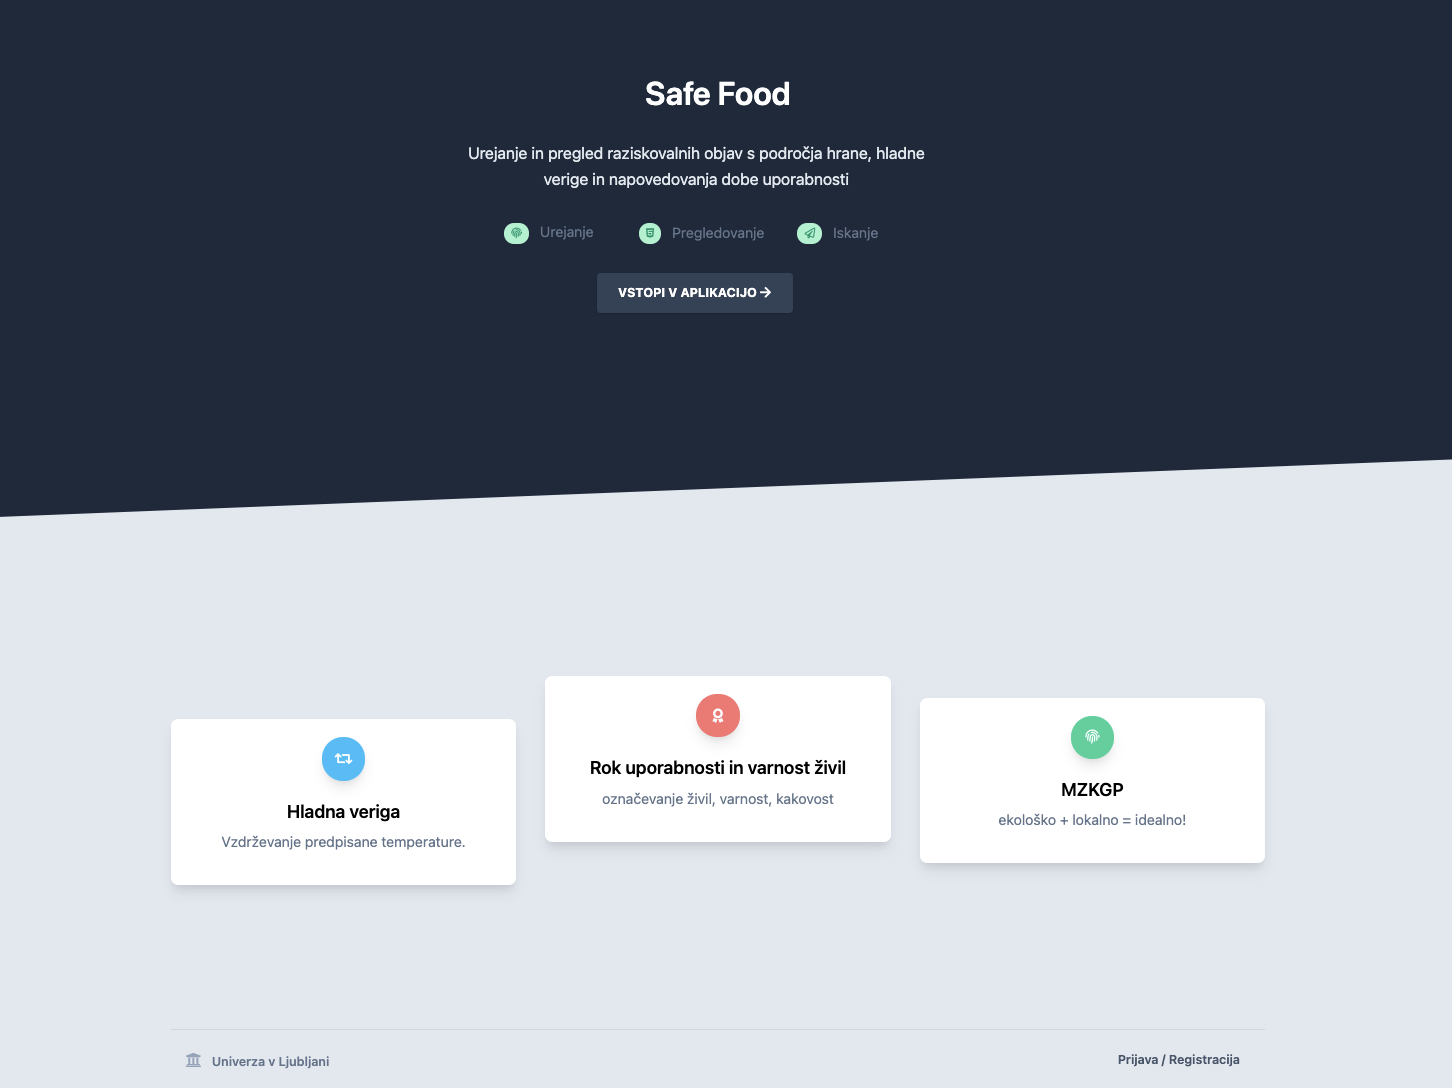
\includegraphics[width=1\textwidth]{slike/landing-page.png}
\end{center}
\caption{ Uvodna stran aplikacije s povezavami na zunanje vire. }
\label{landing-page}
\end{figure}



% #####################################################################
\newpage
% #####################################################################
\section{Prijava uporabnika }
\label{sign-in-page}
Obstoječi uporabnik se lahko prijavi z uporabniškim imenom in geslom (Slika \ref{login-form}. Če je uporabnik presegel določeno število neuspešnih poizkusov prijave, mu je dostop do strani začasno omejen in prijava onemogočena. Na vrhu obrazca se izpiše ustrezna napaka, ki podaja razlog napake in navodila za njeno odpravljanje. Poleg tega lahko uporabnik spodaj klikne \sn{Forgot password}, če je pozabil geslo, ali \sn{Create new account}, če še ni prijavljen. 


% V primeru pozabljenega gesla, lahko s klikom na \sn{Pozabljeno geslo} nadaljujemo na stran, kjer se odpre stran, z obrazcem za ponastavitev gesla (Poglavje \ref{forgotten-form}). 
% Implementirali smo tudi varnostni mehanizem, ki preprečuje uporabniku ugibati gesla. 

\begin{figure}[h]
\begin{center}
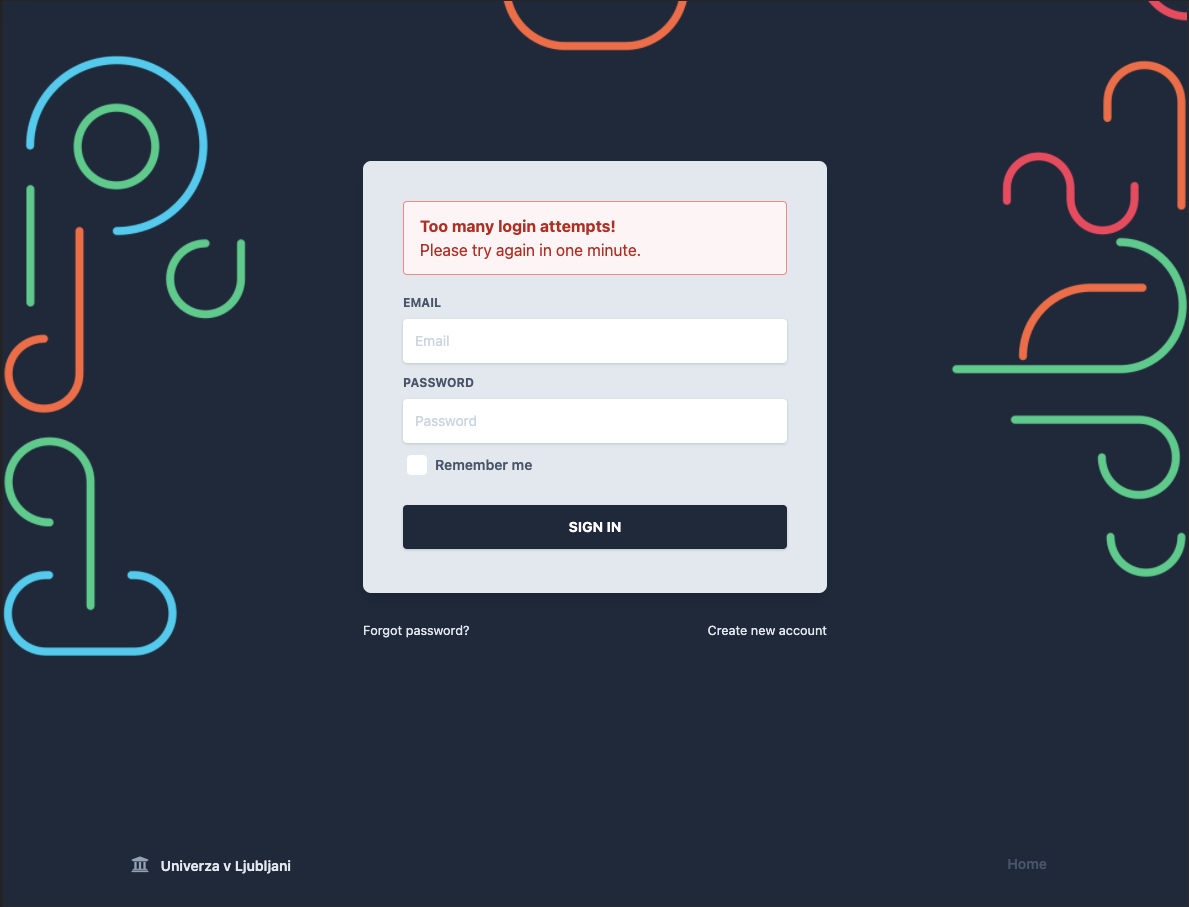
\includegraphics[width=1\textwidth]{slike/signin-throttling.png}
\end{center}
\caption{ Prijava uporabnika in izpis napake v primeru blokiranja uporabnika. }
\label{login-form}
\end{figure}

% #####################################################################
\subsection{Pozabljeno geslo}
\label{forgotten-form}
V primeru, da izgubimo ali pozabimo geslo za prijavo v aplikacijo, na prijavni strani izberemo \sn{Forgot password}. S klikom na gumb se odpre spletni obrazec (Slika \ref{password-reset-form}), kjer vnesemo e-poštni naslov, s katerim smo identificirani v aplikaciji. Na ta naslov prejmemo sporočilo, ki zajema unikatno ustvarjeno URL povezavo do aplikacije. S klikom na povezavo se odpre stran za vnos novega gesla. Ob uspešni nastavitvi gesla je uporabnik preusmerjen na prijavno stran, kjer se mora prijaviti z novim geslom. 

V primeru, da aplikacijo uporabljamo na različnih napravah, nam bo odvzet dostop iz vseh ostalih naprav, kar pomeni, da bo na vseh potrebna ponovna prijava.

\begin{figure}[h]
\begin{center}
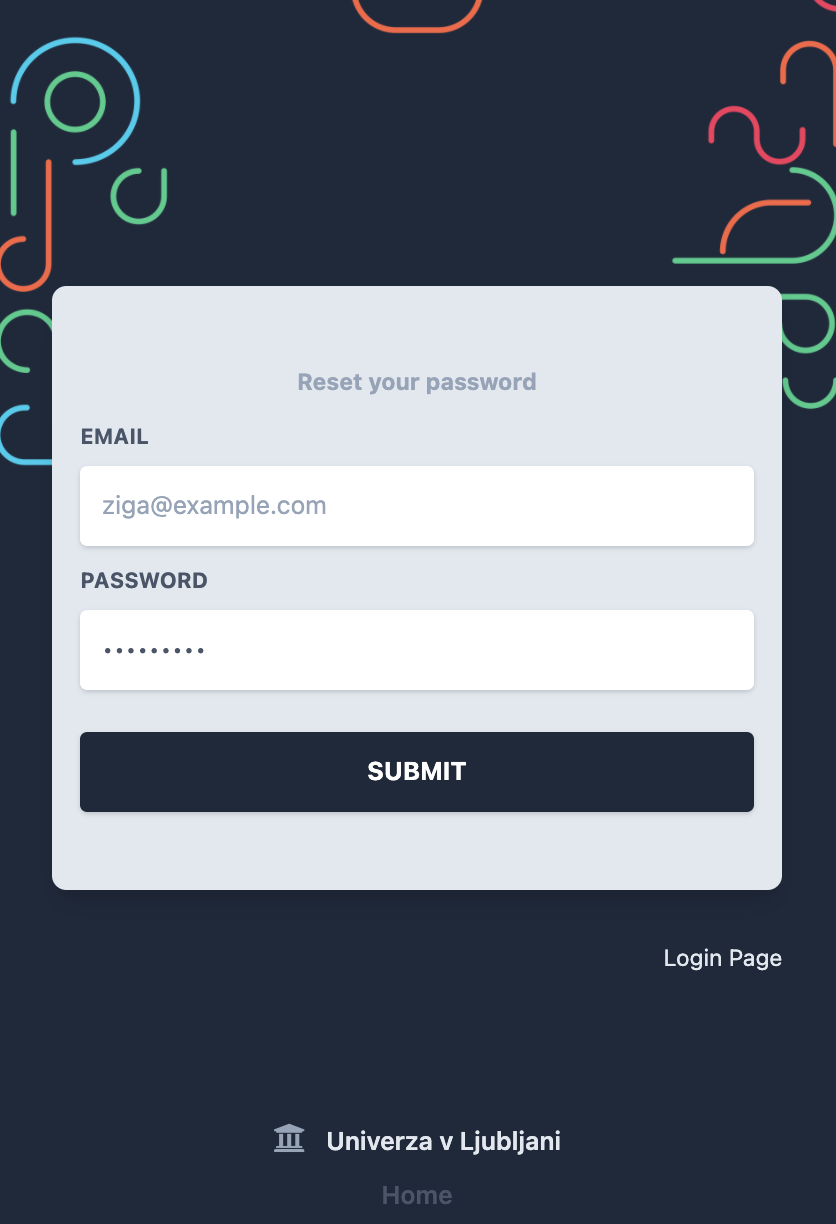
\includegraphics[width=0.5\textwidth]{slike/reset_password.png}
\end{center}
\caption{ Vnos novega gesla. }
\label{password-reset-form}
\end{figure}
% #####################################################################

% #####################################################################
\subsection{Stran za registracijo }
\label{registration-page}
Za uporabo aplikacije je potrebna registracija. Uporabniki, ki še niso registrirani v aplikacijo, imajo možnost, da si ustvarijo račun (Slika \ref{signup-form}). Na strani se nahaja obrazec za vnos potrebnih informacij za ustvarjanje računa.

\begin{figure}[h]
\begin{center}
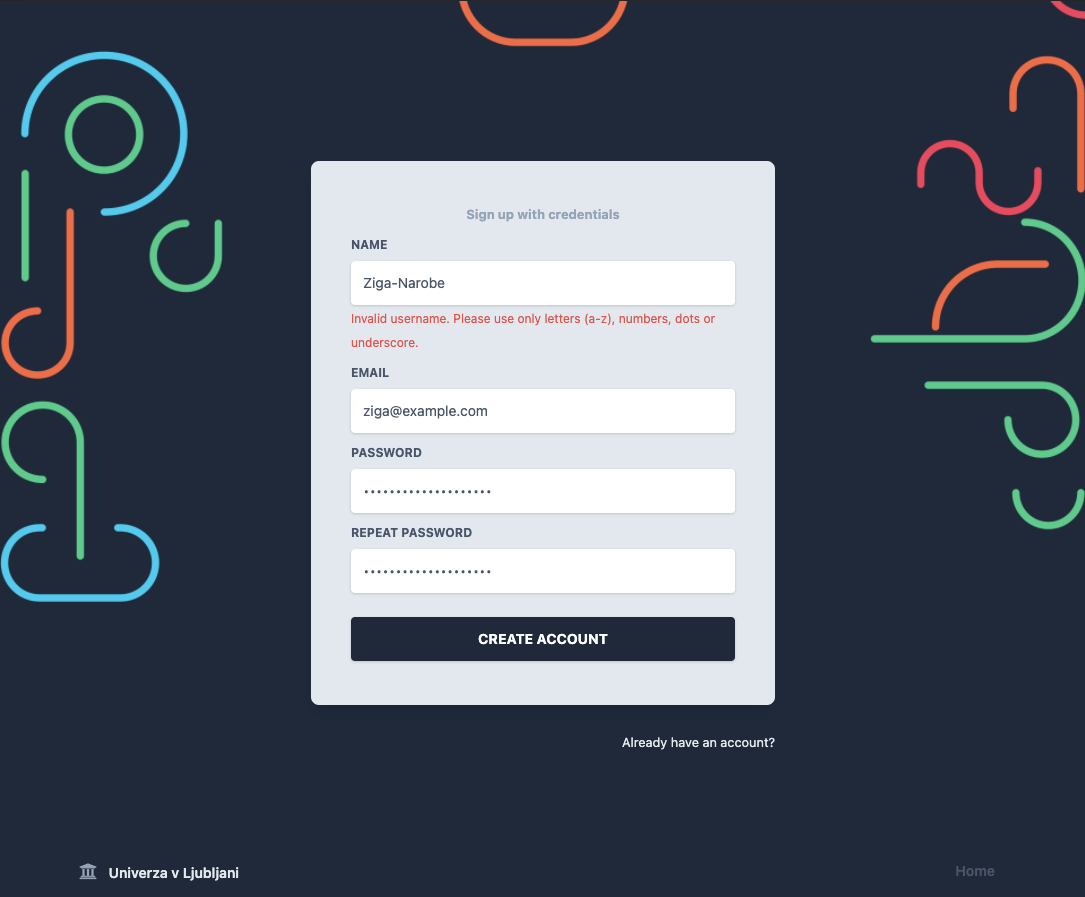
\includegraphics[width=1\textwidth]{slike/signup-validation.png}
\end{center}
\caption{ Registracija uporabnika. }
\label{signup-form}
\end{figure}

Ob kliku na gumb \sn{Create account} se sproži validacija, ki preveri, ali vneseni podatki ustrezajo zahtevam aplikacije. V primeru vnosa napačnega uporabniškega imena, elektronskega naslova ali gesla, se pod posameznim vnosnim poljem izpiše ustrezno opozorilo o napaki. Validacija se izvaja tako na čelnem kot tudi na zalednem delu aplikacije (Koda \ref{lst:validation}). 


\begin{lstlisting}[language=java, style=mystyle,caption={Primer validacijske funkcije za preverjanje uporabniškega imena z uporabo regularnega izraza},label=lst:validation]
function validateUsername(uname) {
  /*
    Uporabnisko ime, ne sme biti krajse od treh znakov
  */
  if(uname.length < 3) {
    return false;
  }

  /* 
    Vsebuje lahko le: 
    - male crke (a-z) 
    - stevilke (0-9)
    - pike (.)
    - podcrtaje (_)
  */
  const match = /^[a-z0-9_\.]+$/.exec(uname);
  
  // veljavno ali ne
  return Boolean(rezultat);
}
\end{lstlisting}

Ob registraciji prejme uporabnik novo sporočilo za potrditev uporabniškega računa. Potrditveno sporočilo je namenjeno zagotavljanju verodostojnosti uporabnika. V primeru, da uporabnik ne potrdi svojega e-poštnega naslova v roku enega dneva, mu je dostop do aplikacije onemogočen, vse dokler ga uporabnik ne potrdi.

Nepotrjen uporabnik nima dostopa do dela aplikacije, kjer so prikazane publikacije. Pokaže se mu le stran z navodili, kako potrditi e-poštni naslov. V primeru, da uporabnik ni prejel potrditvenega sporočila, lahko klikne na gumb in sproži ponovno pošiljanje potrditvenega sporočila. Sporočilo bo ponovno ustvarjeno le v primeru, da je minila vsaj ena ura od zadnjega poizkusa pošiljanja tega sporočila.

Vsak uporabnik je ob registraciji le navaden uporabnik. Vlogo uporabnika lahko spremeni le administrator, v administracijskem delu aplikacije. O tem bomo govorili v poglavju \sn{Administracija uporabnikov} (Poglavje \ref{administracija-uporabnikov}).

V elektronskem sporočilu, ki ga uporabnik prejme na svoj naslov, je navedena povezava do aplikacije. Generirana povezava vsebuje parameter \verb="method"=, ki pove, katera akcija se mora izvesti, ko uporabnik odpre stran. Komponenta prebere parameter $url$ in glede na prebran parameter sproži ustrezno akcijo na storitev za njegovo preverjanje. 

V primeru, da je uporabniški račun uspešno potrjen, je preusmerjen na začetno stran aplikacije, kjer lahko pregleduje objavljene publikacije s pripadajočimi podatki. Zgodi pa se lahko tudi, da elektronski naslov ni uspešno potrjen (Koda \ref{lst:verify-username}). To se lahko zgodi v naslednjih primerih:
\begin{itemize}
  \item potrditvena koda je potekla
  \item potrditvena koda ni veljavna
  \item uporabniški račun je izbrisan
  \item uporabniški račun je onemogočen.
\end{itemize}

% // http://localhost:8080/auth/firebase?mode=resetPassword&oobCode={code}
\begin{lstlisting}[language=bash, style=mystyle,caption={Primer kode, za preverjanje uporabnika.}, label=lst:verify-username]
  mounted() {
    this.mode = queryParams.mode;
    this.oobCode = queryParams.oobCode;

    if (this.mode === "verifyEmail") {
      verifyAccount(this.oobCode).then(() => {
          this.$toast.success("Email verified");
          this.$router.push("home");
        }, (error) => {
          switch (error.code) {
            case 'auth/expired-action-code':
              this.$toast.error('Code expired!')
              break;
            case 'auth/invalid-action-code':
              this.$toast.error('The code is not valid.')
              break
            case 'auth/user-disabled':
              this.$toast.error('Account is disabled, please contact us at support@example.com')
              break
            case 'auth/user-not-found':
              this.$toast.error('Your account has been removed')
              break
            default:
              this.$toast.error('Email verification failed!')
          }
        });
    }
  }
\end{lstlisting}
% #####################################################################


% #####################################################################
\section{Urejanje uporabnikov}
\label{administracija-uporabnikov}
Administrator ima možnost pregledovanja in urejanja uporabnikov v aplikaciji. Na strani \sn{Users List} (Slika \ref{users-list-page}) je seznam registriranih uporabnikov. S klikom na ikono za smeti lahko administrator uporabniku onemogoči račun. Ker je v aplikaciji lahko registriranih veliko uporabnikov, je seznam uporabnikov prikazan na več straneh. Na dnu seznama se nahaja paginacija, s katero lahko prehajamo med stranmi.

\begin{figure}[h]
\begin{center}
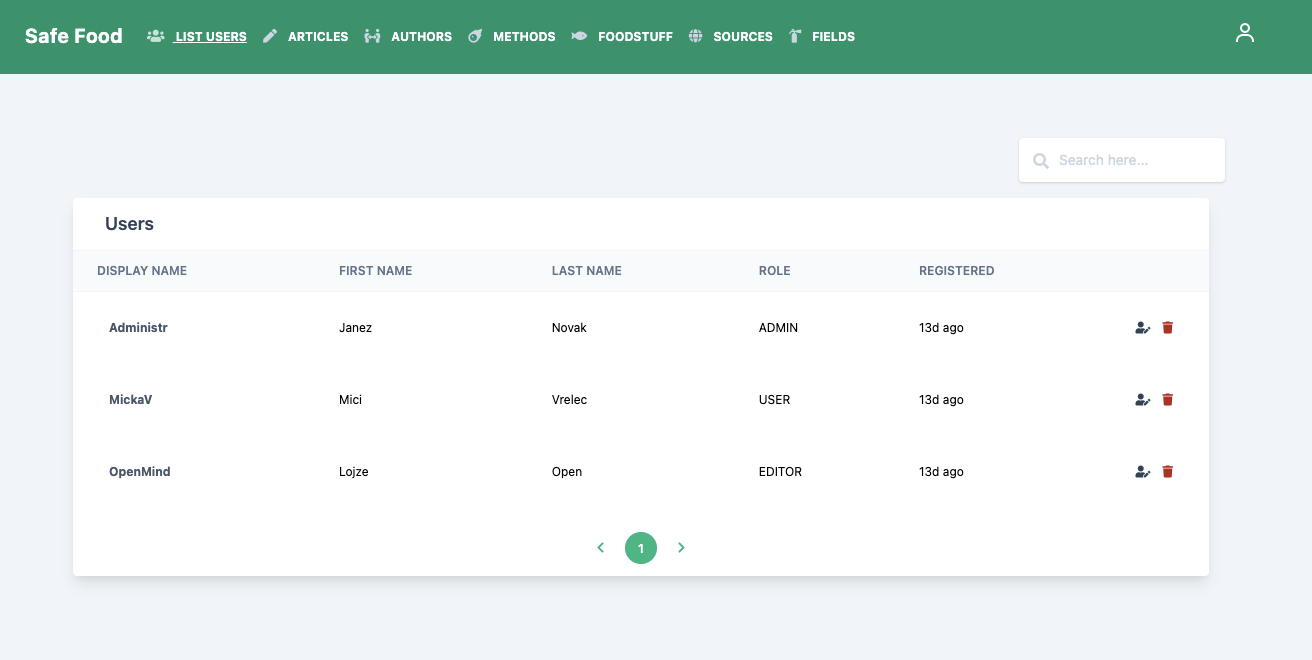
\includegraphics[width=1\textwidth]{slike/users-list.png}
\end{center}
\caption{ Seznam vseh registriranih uporabnikov. }
\label{users-list-page}
\end{figure}

S klikom na ikono za urejanje se odpre stran za urejanje izbranega uporabnika. Na voljo je spreminjanje uporabniškega imena, e-poštnega naslova in ostalih informacij uporabnika, kot sta ime in priimek (Slika \ref{users-edit-page}). 

Administratorju je tudi na voljo spreminjanje vrste uporabnika, torej lahko nekemu uporabniku doda pravice za urednika, ga dodeli kot administratorja, ali pa kot navadnega uporabnika, ki lahko pregleduje vnesene publikacije.

\begin{figure}[h]
\begin{center}
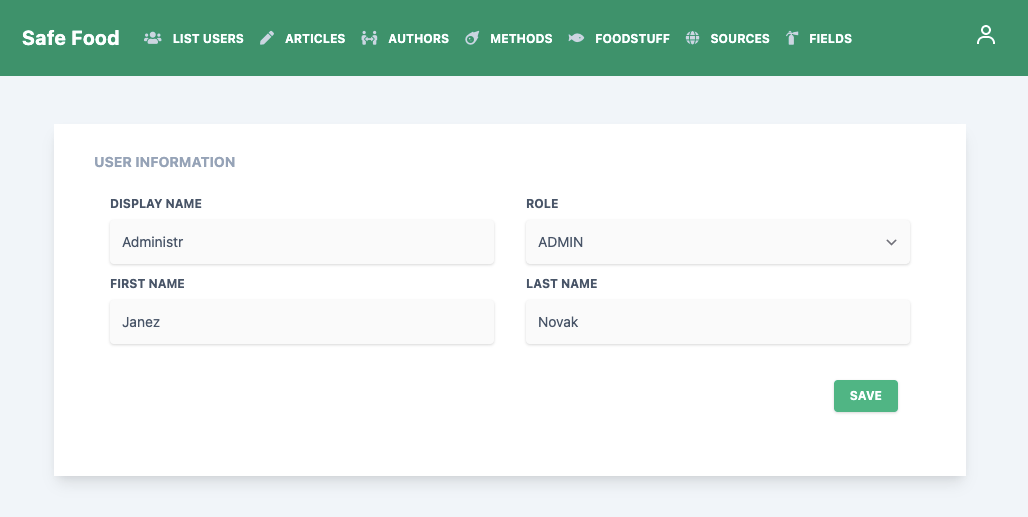
\includegraphics[width=1\textwidth]{slike/users-edit.png}
\end{center}
\caption{ Stran za urejanje uporabnikov. }
\label{users-edit-page}
\end{figure}
% #####################################################################


% #####################################################################
% #####################################################################
\section{Vnos publikacije}
Uredniki s pravicami urejanja ali dodajanja publikacij imajo dostop do strani \sn{Articles}. Na njej je prikazan seznam vseh vnesenih publikacij. Ker je vsako publikacijo mogoče urediti ali izbrisati, se na desni strani nahaja polje z ikonama za urejanje in brisanje posamezne publikacije. 

V primeru, da je vnesenih publikacij veliko, je na dnu seznama na voljo paginacija, s katero se pomikamo med stranmi. Na vrhu seznama imamo tudi možnost iskanja po naslovu publikacije. Seznam publikacij je prikazan z novejšimi publikacijami na vrhu (Slika \ref{list-articles}). Na strani se nahaja tudi gumb za dodajanje nove publikacije (+Add).

\begin{figure}[h]
\begin{center}
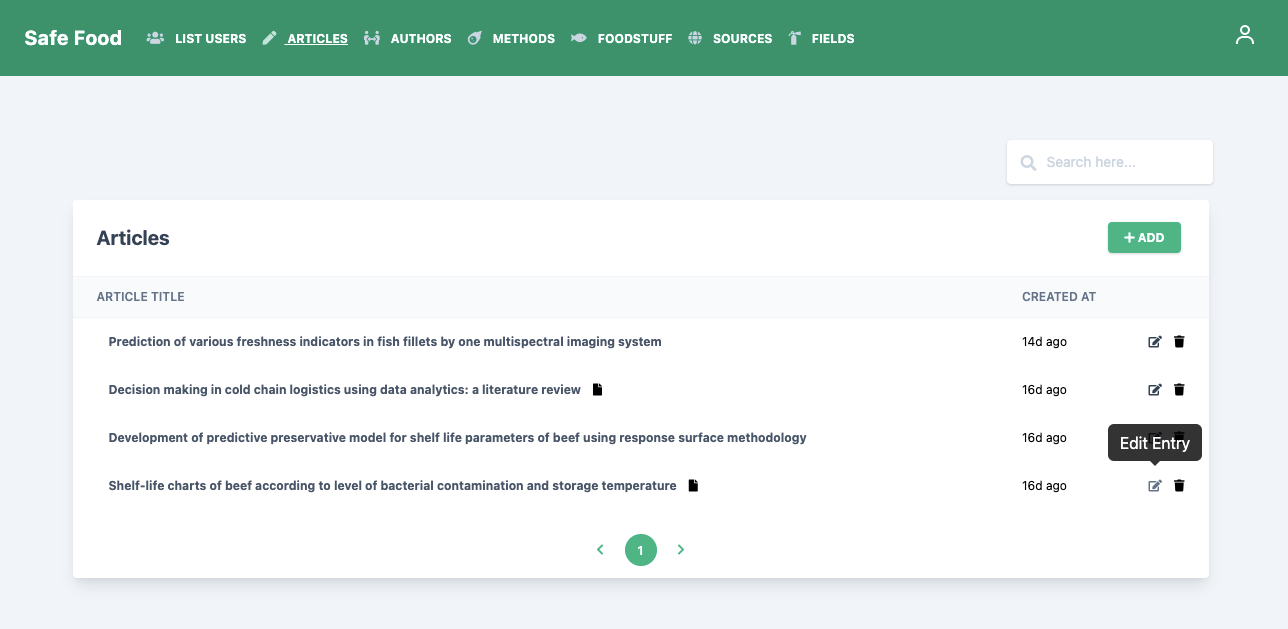
\includegraphics[width=1\textwidth]{slike/list-articles.png}
\end{center}
\caption{ Seznam publikacij v administraciji. }
\label{list-articles}
\end{figure}

S klikom na ikono za urejanje se odpre stran z izpolnjenim spletnim obrazcem s podatki o vneseni publikaciji (Slika \ref{edit-articles}). V ozadju se uporablja ista \verb=vue.js= komponenta tudi za kreiranje nove publikacije. Glede na akcijo je potrebno poslati ustrezen zahtevek na zaledni sistem.

\begin{figure}[h]
\begin{center}
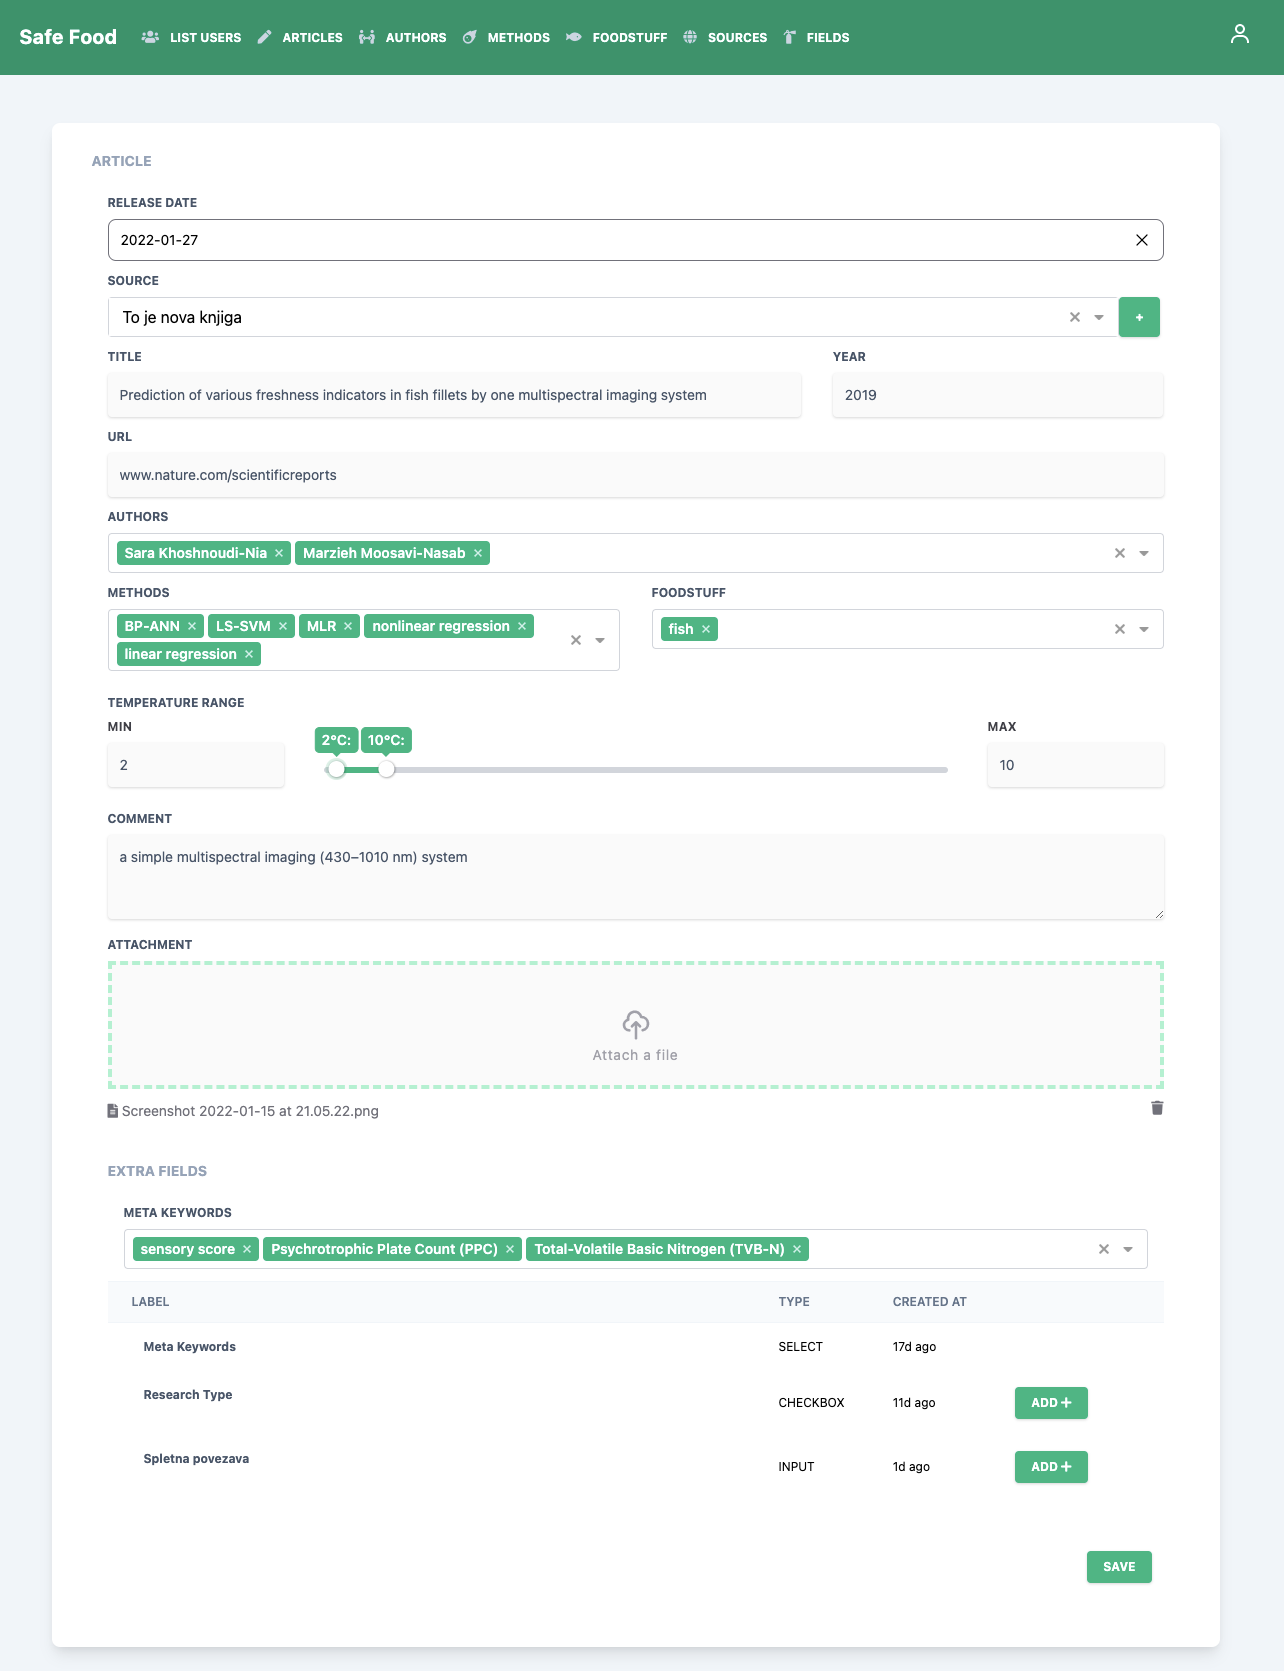
\includegraphics[width=1\textwidth]{slike/form-create-article.png}
\end{center}
\caption{ Spletni obrazec za urejanje ali vnos nove publikacije. }
\label{edit-articles}
\end{figure}

V primeru urejanja, se v naslovu URL nahaja identifikator publikacije, ki jo urejamo. Z njegovo uporabo pošljemo zahtevek na zaledni sistem, kjer dobimo vse potrebne informacije, ki so bile vnesene za dano publikacijo. Ob nalaganju spletnega obrazca moramo zagotoviti še ostale podatke kot so avtorji, metode, živila, viri, in dinamični podatki, katere je uporabnik definiral naknadno. Za vse te podatke imamo na voljo posamezne vire API, na katere pošljemo zahtevek za pridobitev teh podatkov. 

\clearpage
Na spletnem obrazcu je mogoče dodajati in urejati naslednje podatke:

\begin{description}
    \item \textbf{Datum objave} - polje za vpis datuma, ki določa kdaj naj bo publikacija na voljo ostalim uporabnikom. Ta parameter je na voljo le administratorjem.
    
    \item \textbf{Vir} - izbirno polje za izbiro vira, na katerega se nanaša publikacija. S klikom na polje se odpre spustno okno z vnaprej vnesenimi viri. Imamo tudi možnost iskanja vira po njegovem naslovu. V primeru, da vir še ne obstaja, imamo na voljo gumb za dodajanje (+) novega vira. S klikom na gumb se odpre okno za kreiranje novega vira (Slika \ref{add-source}). Ob shranjevanju vira se samodejno izpolni polje z virom, ki je bil na novo vnesen.
    
    \begin{figure}[h]
        \begin{center}
        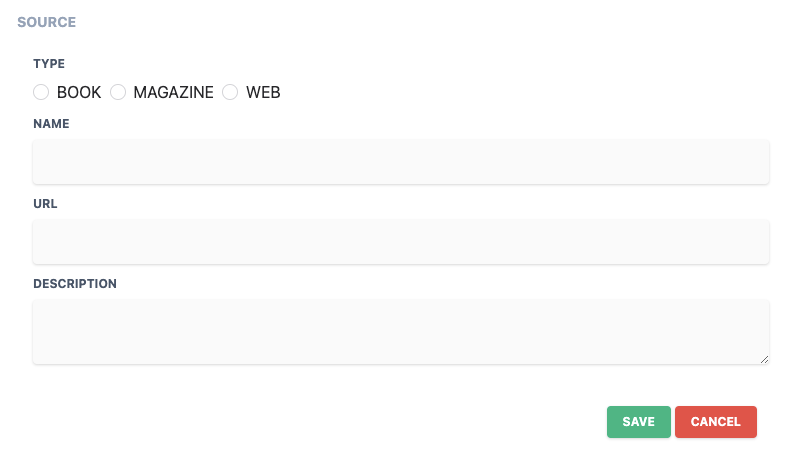
\includegraphics[width=0.75\textwidth]{slike/add-source.png}
        \end{center}
        \caption{ Obrazec za dodajanje novega vira. }
        \label{add-source}
    \end{figure}
    
    \item \textbf{Naslov} - tekstovno polje, ki vsebuje naslov publikacije.
    
    \item \textbf{Leto} - numerično polje, ki vsebuje leto izdaje publikacije.
    
    \item \textbf{Spletni vir} - povezava na vir, kjer lahko pridobimo več informacij o publikaciji.
    
    \item \textbf{Avtorji} - izbirno polje za izbiro enega ali več avtorjev. Ob kliku na polje se odpre spustni meni s seznamom avtorjev po katerih lahko izvajamo iskanje. V primeru, da avtor ne obstaja, imamo možnost dodajanja novega avtorja z vpisom njegovega imena. Ob potrditvi bo avtor avtomatsko dodan v zalednem sistemu in izbran v izbirnem polju.
    
    \item \textbf{Metode} - uporablja se enaka komponenta kot pri polju za izbiro avtorjev, le da se v tem primeru izbirajo metode. 
    
    \item \textbf{Živila} - uporablja se enaka komponenta kot pri polju za izbiro avtorjev, le da se v tem primeru izbirajo živila (Slika \ref{multiselect}).
    
    \begin{figure}[h]
        \begin{center}
        
\includegraphics[width=0.5\textwidth]{slike/multiselect.png}
        \end{center}
        \caption{ Spustni meni s predlaganimi vrednostmi. }
        \label{multiselect}
    \end{figure}
    
    \item \textbf{Temperaturno območje} - predstavlja območje dveh števil, katerega je mogoče izbrati s horizontalnim drsnikom, ali pa z vpisom vrednosti v posamezna polja (minimalno in maksimalno vrednost v °C) (Slika  \ref{type-range}).
    
    \begin{figure}[h]
        \begin{center}
        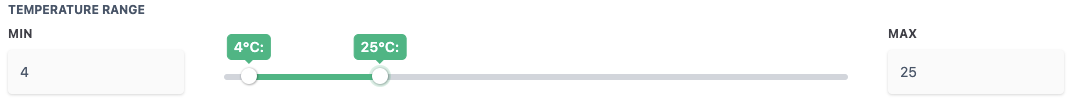
\includegraphics[width=1\textwidth]{slike/type_range.png}
        \end{center}
        \caption{ Komponenta za določanje vrednosti v območju. }
        \label{type-range}
    \end{figure}
    
    \item \textbf{Komentar} - tekstovno polje, kjer je mogoče vnesti daljše besedilo, do 255 znakov.
    
    \item \textbf{Priponka} - polje za odlaganje datoteke. Na voljo je izbira datotek, ki se pripne k publikaciji. Prikaže se znotraj komponente in jo je mogoče odstraniti (Slika  \ref{type-fileupload}).
    
    \begin{figure}[h]
    \begin{center}
        
\includegraphics[width=1\textwidth]{slike/upload_file_zone.png}
        
\includegraphics[width=1\textwidth]{slike/upload_file_list.png}
        \end{center}
        \caption{ Komponenta za nalaganje datotek. }
        \label{type-fileupload}
    \end{figure}
  
    \item \textbf{Dodatna polja} - seznam dodatnih polj, ki jih želimo dodati k publikaciji. Ob kliku nanje se pojavi možnost za definiranje vrednosti tega podatka. Vnosno polje se prikaže različno glede na tip podatka, ki ga izberemo (Slika \ref{fields-usage}).
    \begin{figure}[h]
        \begin{center}
        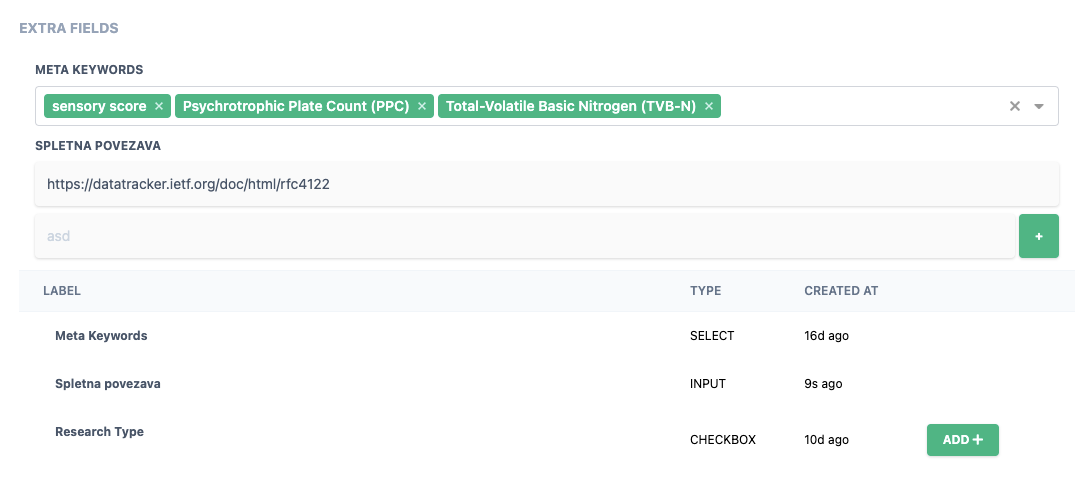
\includegraphics[width=1\textwidth]{slike/fields_usage.png}
        \end{center}
        \caption{ Prikaz uporabe dodanega parametra, med urejanjem publikacije. }
        \label{fields-usage}
    \end{figure}
   
\end{description}

S klikom na gumb \sn{Save}, ki se nahaja spodaj desno, sprožimo zahtevek za shranjevanje vnesenih podatkov. Osnovna validacija se izvaja že med samim vnosom podatkov na čelnem delu. V primeru napačnega vnosa podatkov se na obrazcu poleg posameznih vnosnih polj prikaže sporočilo z opisom napake. Ob uspešnem shranjevanju se pokaže sporočilo, da je bila publikacija uspešno shranjena. 


% #####################################################################
% #####################################################################
% #####################################################################
\section{Prikaz publikacije}
Publikacija je na strani vizualno predstavljena z vso vneseno vsebino. Na vrhu je napisan naslov publikacije, ki je podan kot odebeljeno besedilo, saj je najbolj pomemben podatek za uporabnika. Pod naslovom so izpisani vsi avtorji, ki so sodelovali pri publikaciji. Vsak podatek je predstavljen z imenom in nato s svojo vrednostjo (Slika \ref{publicitation-info}).

Sledijo podatki o sami publikaciji. Vir je predstavljen s tipom, imenom in povezavo, če jo ima. V primeru, da spletna povezava ni bila vnesena le-ta ni prikazana. Ker je lahko vnesenih metod in živil za posamezno publikacijo mnogo, so prikazane kot vrednosti, ločene z vejico. Na skrajno desni strani je predstavljena vrednost temperature, v primeru, da je ta definirana za posamezno publikacijo. 

Publikacija lahko vsebuje tudi komentar, ki je prikazan kot daljše tekstovno polje. Poleg komentarja se nahajajo še ostale povezave do zunanjih virov, če so bili vneseni med samim vnosom publikacije. V primeru, da ima publikacija pripete datoteke, se prikažejo kot ikona datoteke. S klikom na ikono se nam odpre novo okno s povezavo do datoteke. Datoteka je posredovana preko zalednega sistema in jo je mogoče prenesti v samem brskalniku.


\begin{figure}[h]
\begin{center}
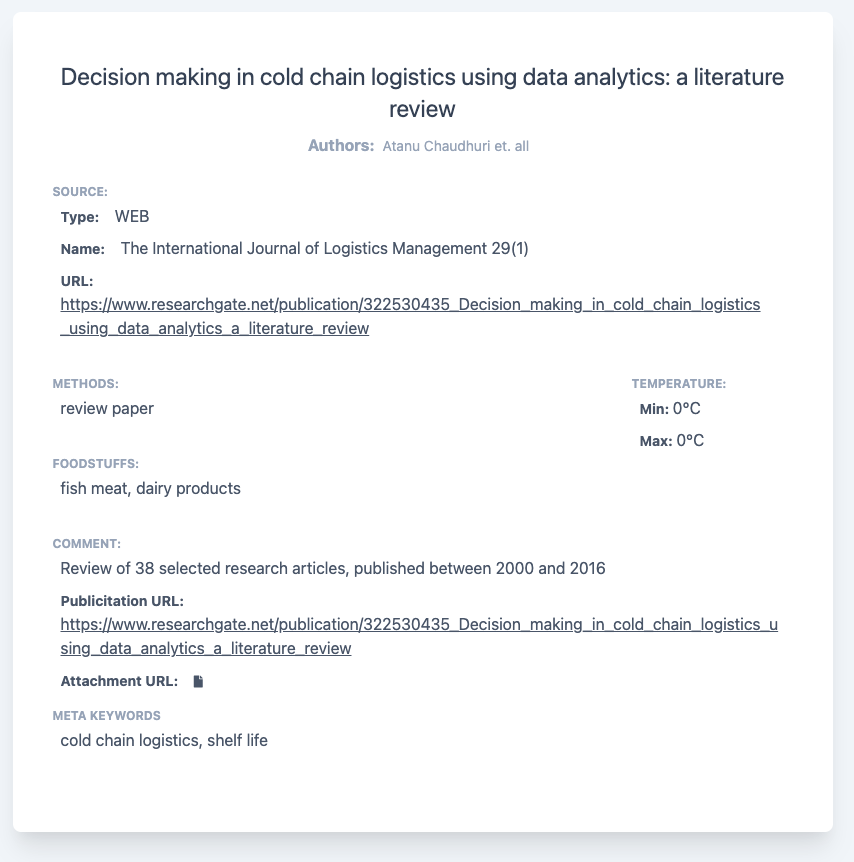
\includegraphics[width=1\textwidth]{slike/publicitation-info.png}
\end{center}
\caption{ Prikaz publikacije z vnesenimi podatki o avtorjih, metodah in ostalih podatkov. }
\label{publicitation-info}
\end{figure}

\clearpage
% #####################################################################

% #####################################################################
% #####################################################################
% #####################################################################
\section{Iskanje publikacij}
\label{filters-page}
Vse vnesene publikacije so uporabniku prijazno prikazane na eni strani. Za pregledovanje ima na voljo številne filtre, kar mu omogoča, da s tem hitreje najde publikacijo, ki jo išče. Iskanje je omogočeno po vseh možnih podatkih, vnesenih za posamezno publikacijo. 


Stran je razdeljena na dva dela. Na levem delu so uporabniku na voljo filtri, katere lahko uporabi za iskanje po publikacijah, na desnem delu pa se uporabniku te publikacije prikažejo. V primeru, da je najdenih publikacij za izbrane filtre veliko, imamo na dnu možnost sprehajanja med posameznimi stranmi, na vrhu pa se izpiše število vseh publikacij, ki ustrezajo izbranim filtrom.


Uporaba filtrov je enostavna. Na levem delu so izpisani vsi podatki, po katerih je mogoče iskati. Ob kliku na filter se prikaže nabor vrednosti, katere lahko uporabnik izbira, in s tem vklopi ali izklopi filter. V zgornjem delu strani je na voljo tudi iskanje po tekstovnem nizu besed, kjer uporabnik vnese niz za izvedbo filtriranja. Vsebina na strani se samodejno osveži in prikaže publikacije, ki ustrezajo izbranim filtrom. 


\begin{figure}[h]
\begin{center}

\includegraphics[width=1\textwidth]{slike/search.png}
\end{center}
\caption{ Praktični prikaz uporabe filtrov na strani za iskanje publikacij. }
\label{seach-example}
\end{figure}

Na sliki \ref{seach-example} je prikazana praktična uporaba filtrov. V njihovi kombinaciji smo dobili rezultat, ki upošteva vse naštete filtre. 

% #####################################################################
% ############ Sklepne ugotovitve #####################################
% #####################################################################

% #####################################################################
\chapter{Sklepne ugotovitve}
% Sklepne ugotovitve lahko zaˇcnete z enim odstavkom opisa, kaj je bilo v
% diplomski nalogi narejenega in kaj so bili njeni glavni prispevki. Sledi naj
% nekaj odstavkov, kjer opiˇsete, zakaj so ti prispevki lahko pomembni, kakˇsna
% je njihova moˇzna uporaba in kaj bi bilo moˇzno v zvezi z zastavljenimi cilji
% v diplomi ˇse storiti oz. izboljˇsati. Ce se razvito delo ˇze uporablja, to nujno ˇ
% omenite v tem poglavju in morda opiˇsite, kakˇsni so odzivi oziroma izkuˇsnje
% uporabnikov

Med razvojem aplikacije, ki smo jo opisali skozi celotno diplomsko delo, sem se hotel naučiti čim več. Spoznal sem nov programski jezik - \verb=Go= in nov arhitekturni koncept mikrostoritev (angl. microservice). Omenjeni dve stvari sta me dodatno spodbudili k delu in spoznavanju novih stvari na področju razvoja programske opreme in pa tudi same organizacije dela.

Z vpeljavo arhitekturnega koncepta mikrostoritev je bila izdelana spletna aplikacija. Pri izdelavi diplomske naloge je bil upoštevan celoten postopek, od ideje in načrtovanja, do same izvedbe in testiranja aplikacije. Pri njenem razvoju in izvedbi smo se soočili z različnimi omejitvami in težavami, katere smo uspešno odpravili in zagotovili, da aplikacija deluje hitro in brez napak. 

Nadaljnji razvoj aplikacije bi lahko potekal v smeri brezglavega urejevalnika vsebin, kar pomeni, da bi zasnovali aplikacijski vmesnik za dinamično urejanje podatkov. Zaradi arhitekturne zasnove je enostavno izluščiti del dinamičnega dodajanja podatkov. Z novo storitvijo, ki bi skrbela za definiranje, shranjevanje, urejanje in brisanje dinamičnih podatkov bi prišli do rešitve, ki bi podpirala uporabo za različne vrste podatkov, ne samo za naš trenutni primer, to je za vnašanje publikacij. 

Razvili bi lahko tudi novo storitev s katero bi avtomatizirali vnašanje podatkov v aplikacijo. Ta bi skrbela za pridobivanje publikacij iz različnih virov (API) in jih preko aplikacijskega vmesnika vnašala v našo aplikacijo. Dodali bi lahko še izvoz in generiranje ustreznega dokumenta za publikacijo.

% \newpage %dodaj po potrebi, da bo številka strani za Literaturo v Kazalu pravilna!
% \\
\clearpage
\addcontentsline{toc}{chapter}{Literatura}
\bibliographystyle{plain}
\bibliography{diploma}


\end{document}

